\documentclass[a4paper,12pt]{article}
\usepackage{tabularx}
\usepackage[utf8]{inputenc}
\usepackage{graphicx}
\usepackage{geometry}
\usepackage{rotating}
\usepackage{seqsplit}
\usepackage{longtable}
\usepackage{booktabs}
\usepackage{caption}
\usepackage{float}
\usepackage{hyperref}
\usepackage{pdflscape}
\usepackage{array}
\usepackage{xcolor}
\usepackage{siunitx}
\newcolumntype{C}[1]{>{\centering\arraybackslash}m{#1}}
\graphicspath{{../figures/}}

\newcommand{\bibcommenthead}{}

\geometry{left=2.5cm, right=2.5cm, top=2.500cm, bottom=2.5cm}

\title{Supplementary Materials for:\\
\textbf{C1Q/SPP1 Macrophage Spatial Context as a Reproducible Traceability Feature in Non-Small Cell Lung Cancer}}
\author{}
\date{}

\renewcommand{\thefigure}{S\arabic{figure}}
\renewcommand{\thetable}{S\arabic{table}}
\setcounter{figure}{0}
\setcounter{table}{0}

\begin{document}

\maketitle

\tableofcontents

\newpage

\section{Supplementary Figures}

\begin{figure}[H]
  \centering
  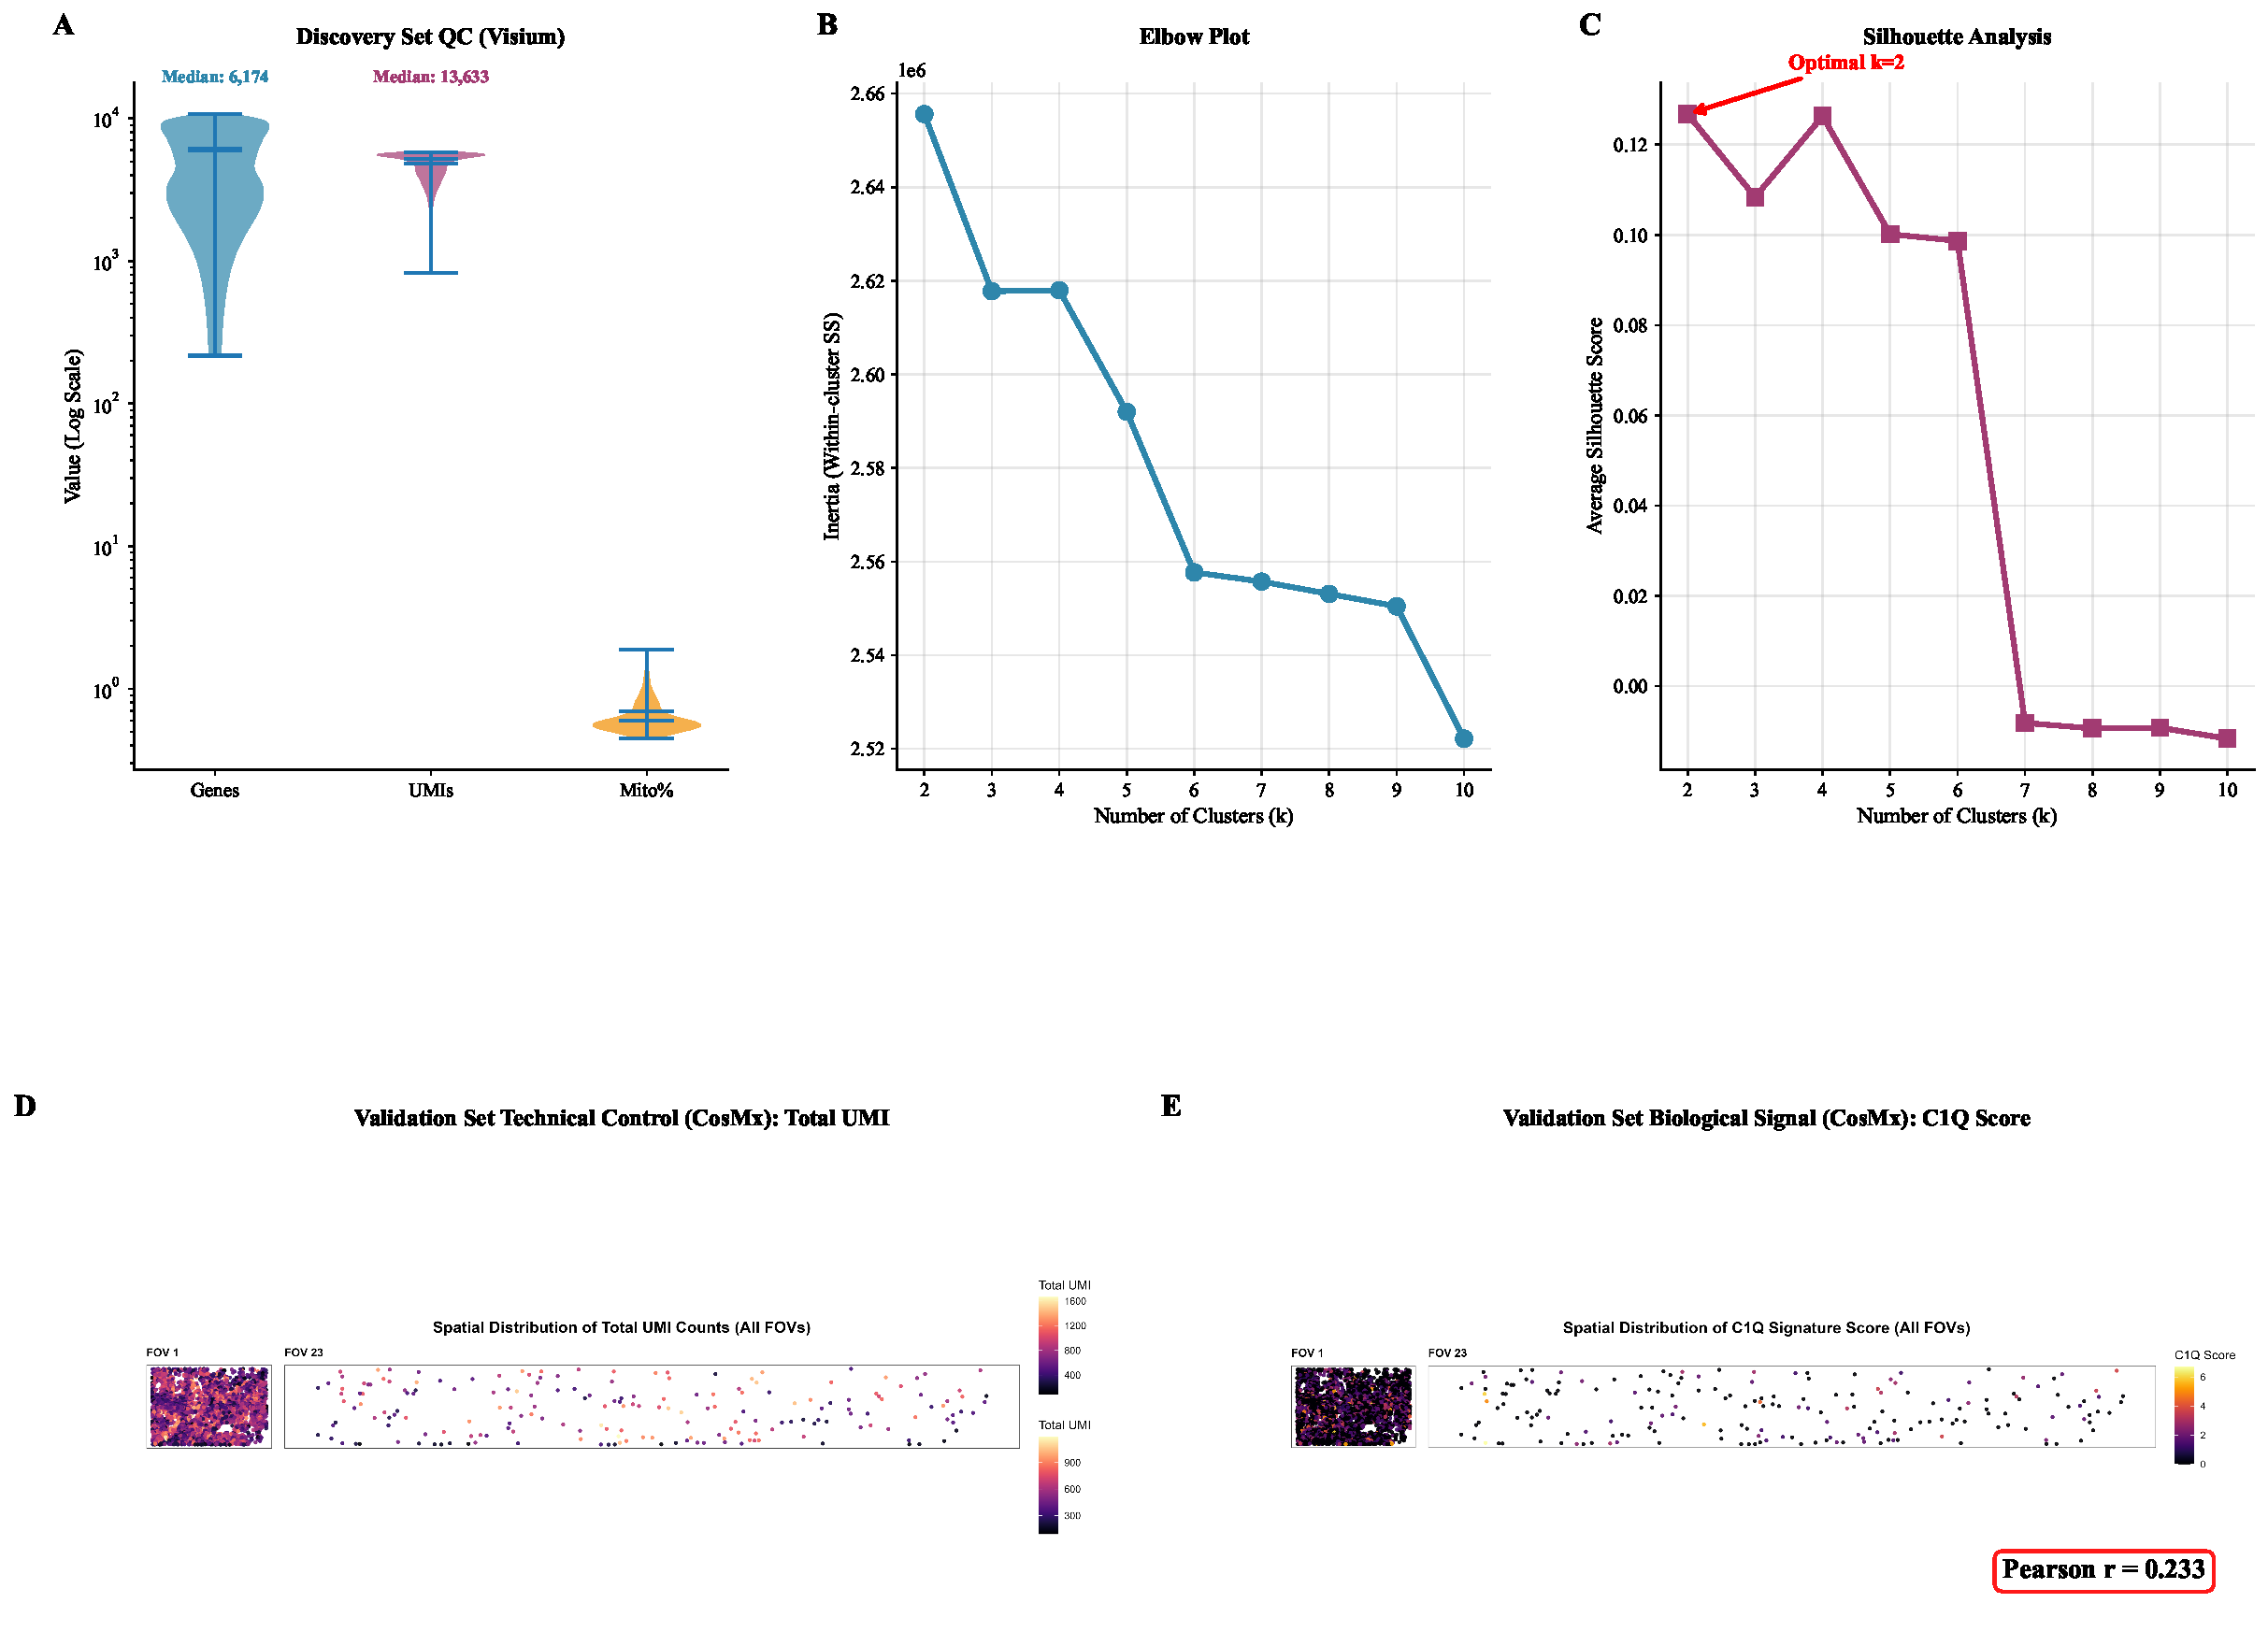
\includegraphics[width=0.95\textwidth]{FigureS1.pdf}
  \caption{\textbf{Quality control and clustering analysis of spatial transcriptomics data.} (A) Violin plots displaying quality control metrics (nFeature, nCount, percent.mt) for spatial spots across the tissue section. (B) UMAP visualization of spatial spots colored by identified clusters. (C) Spatial distribution of clusters on the tissue section. (D) Heatmap of top marker gene expression across clusters.}
  \label{fig:S1}
\end{figure}

\begin{figure}[H]
  \centering
  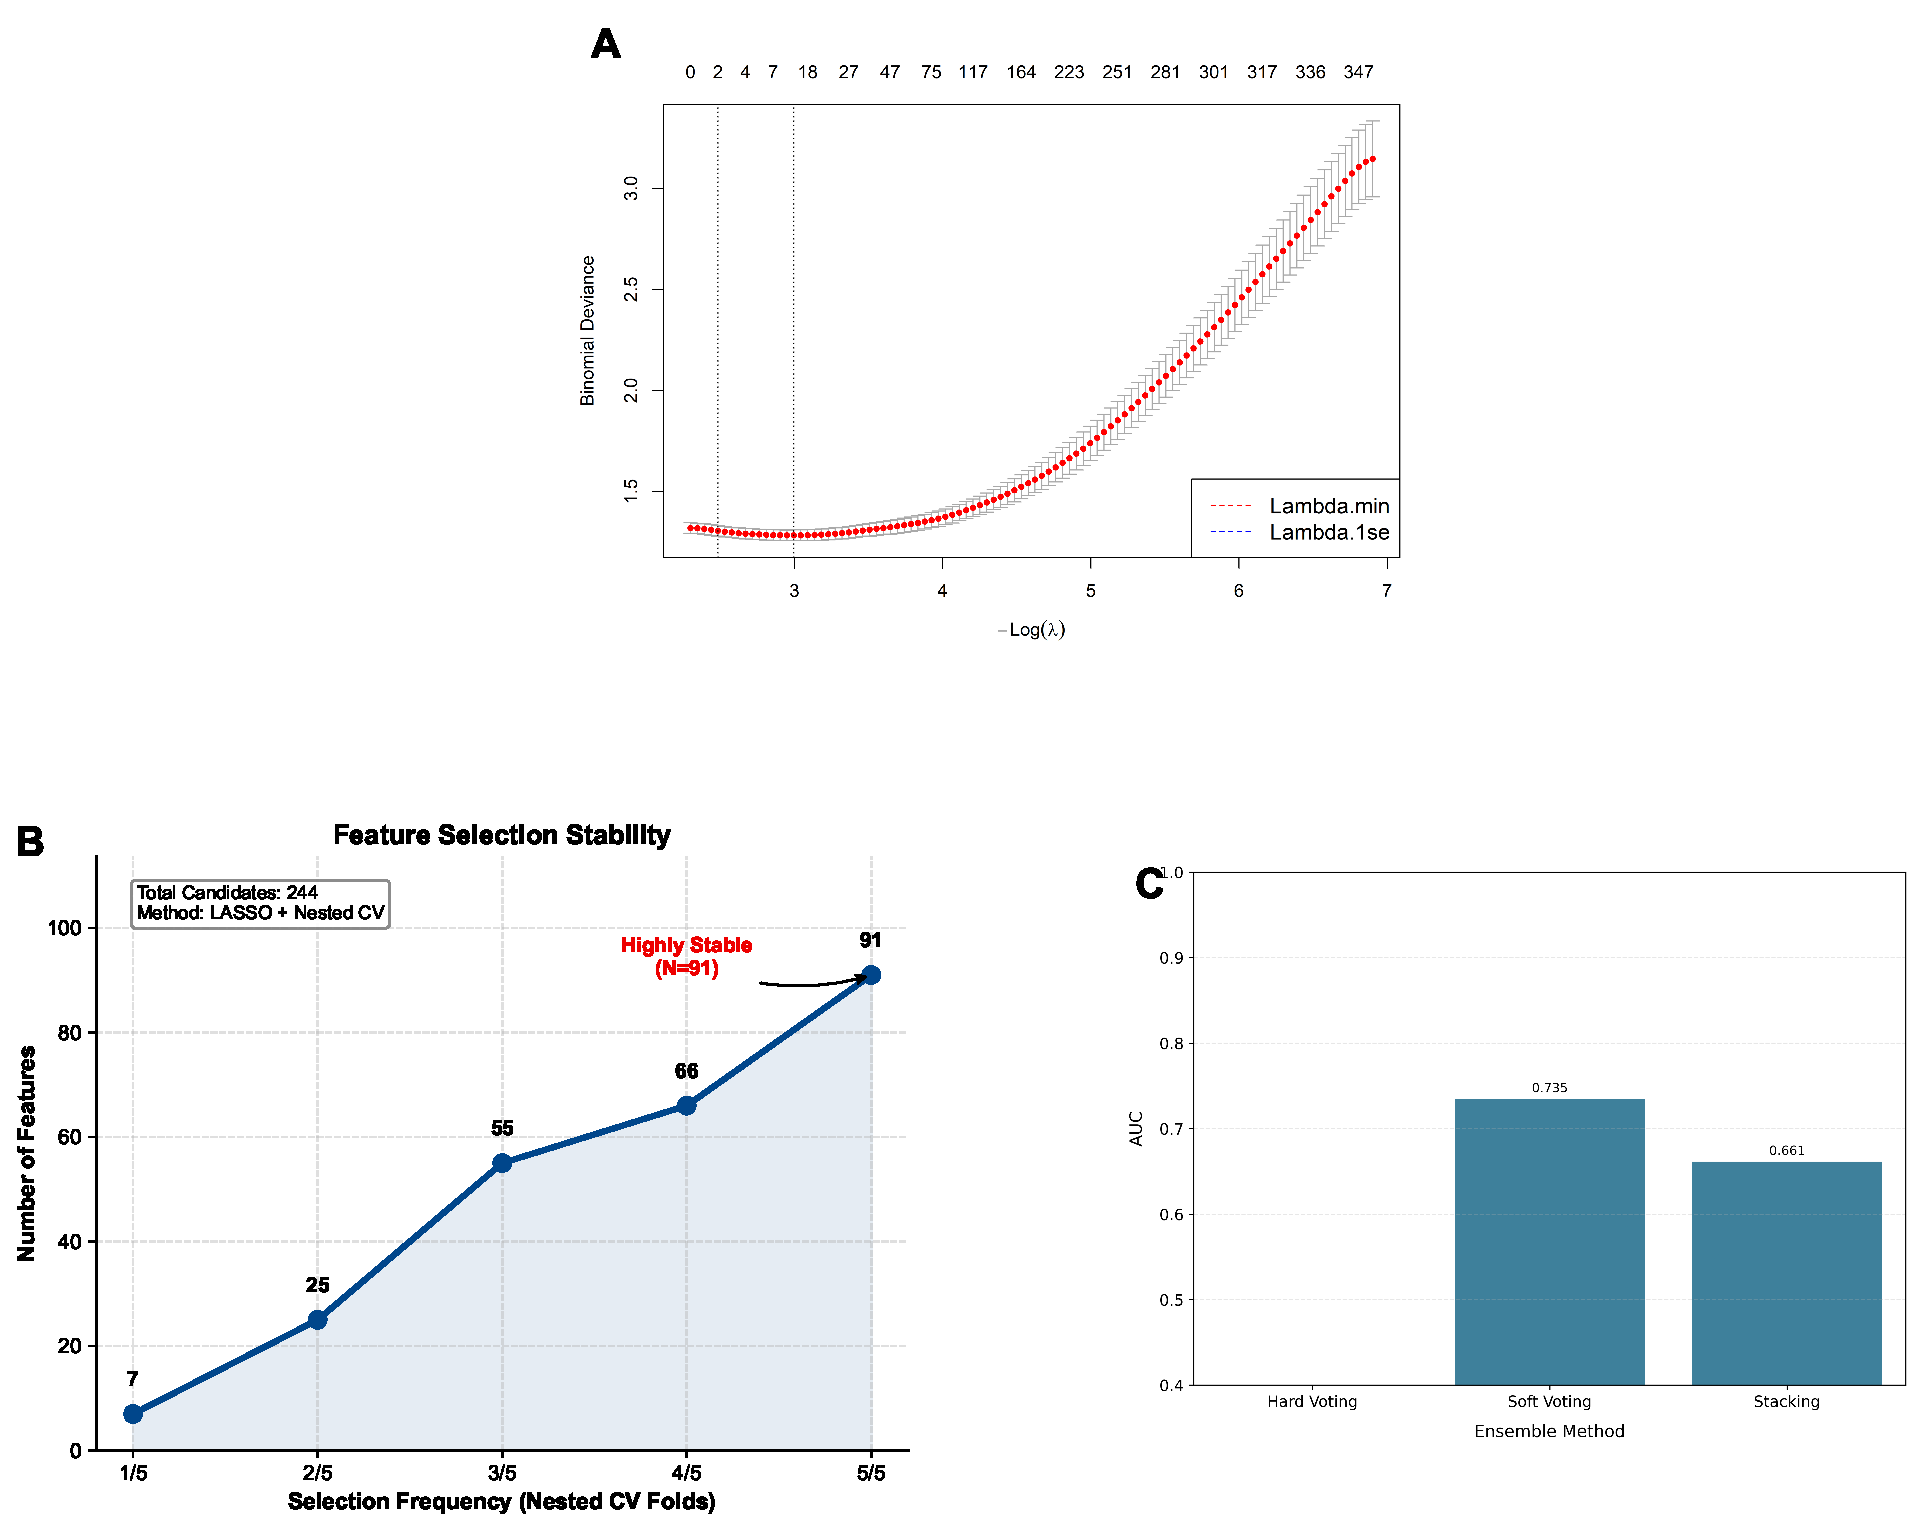
\includegraphics[width=0.95\textwidth]{FigureS2.pdf}
  \caption{\textbf{Machine learning model development and internal assessment details.} (A) Learning curves showing training and cross-validation scores for increasing training set sizes. (B) Feature selection stability analysis using SelectKBest with f\_classif. (C) Hyperparameter optimization results grid search performance. (D) Distribution of performance metrics across 5-fold cross-validation.}
  \label{fig:S2}
\end{figure}

\begin{figure}[H]
  \centering
  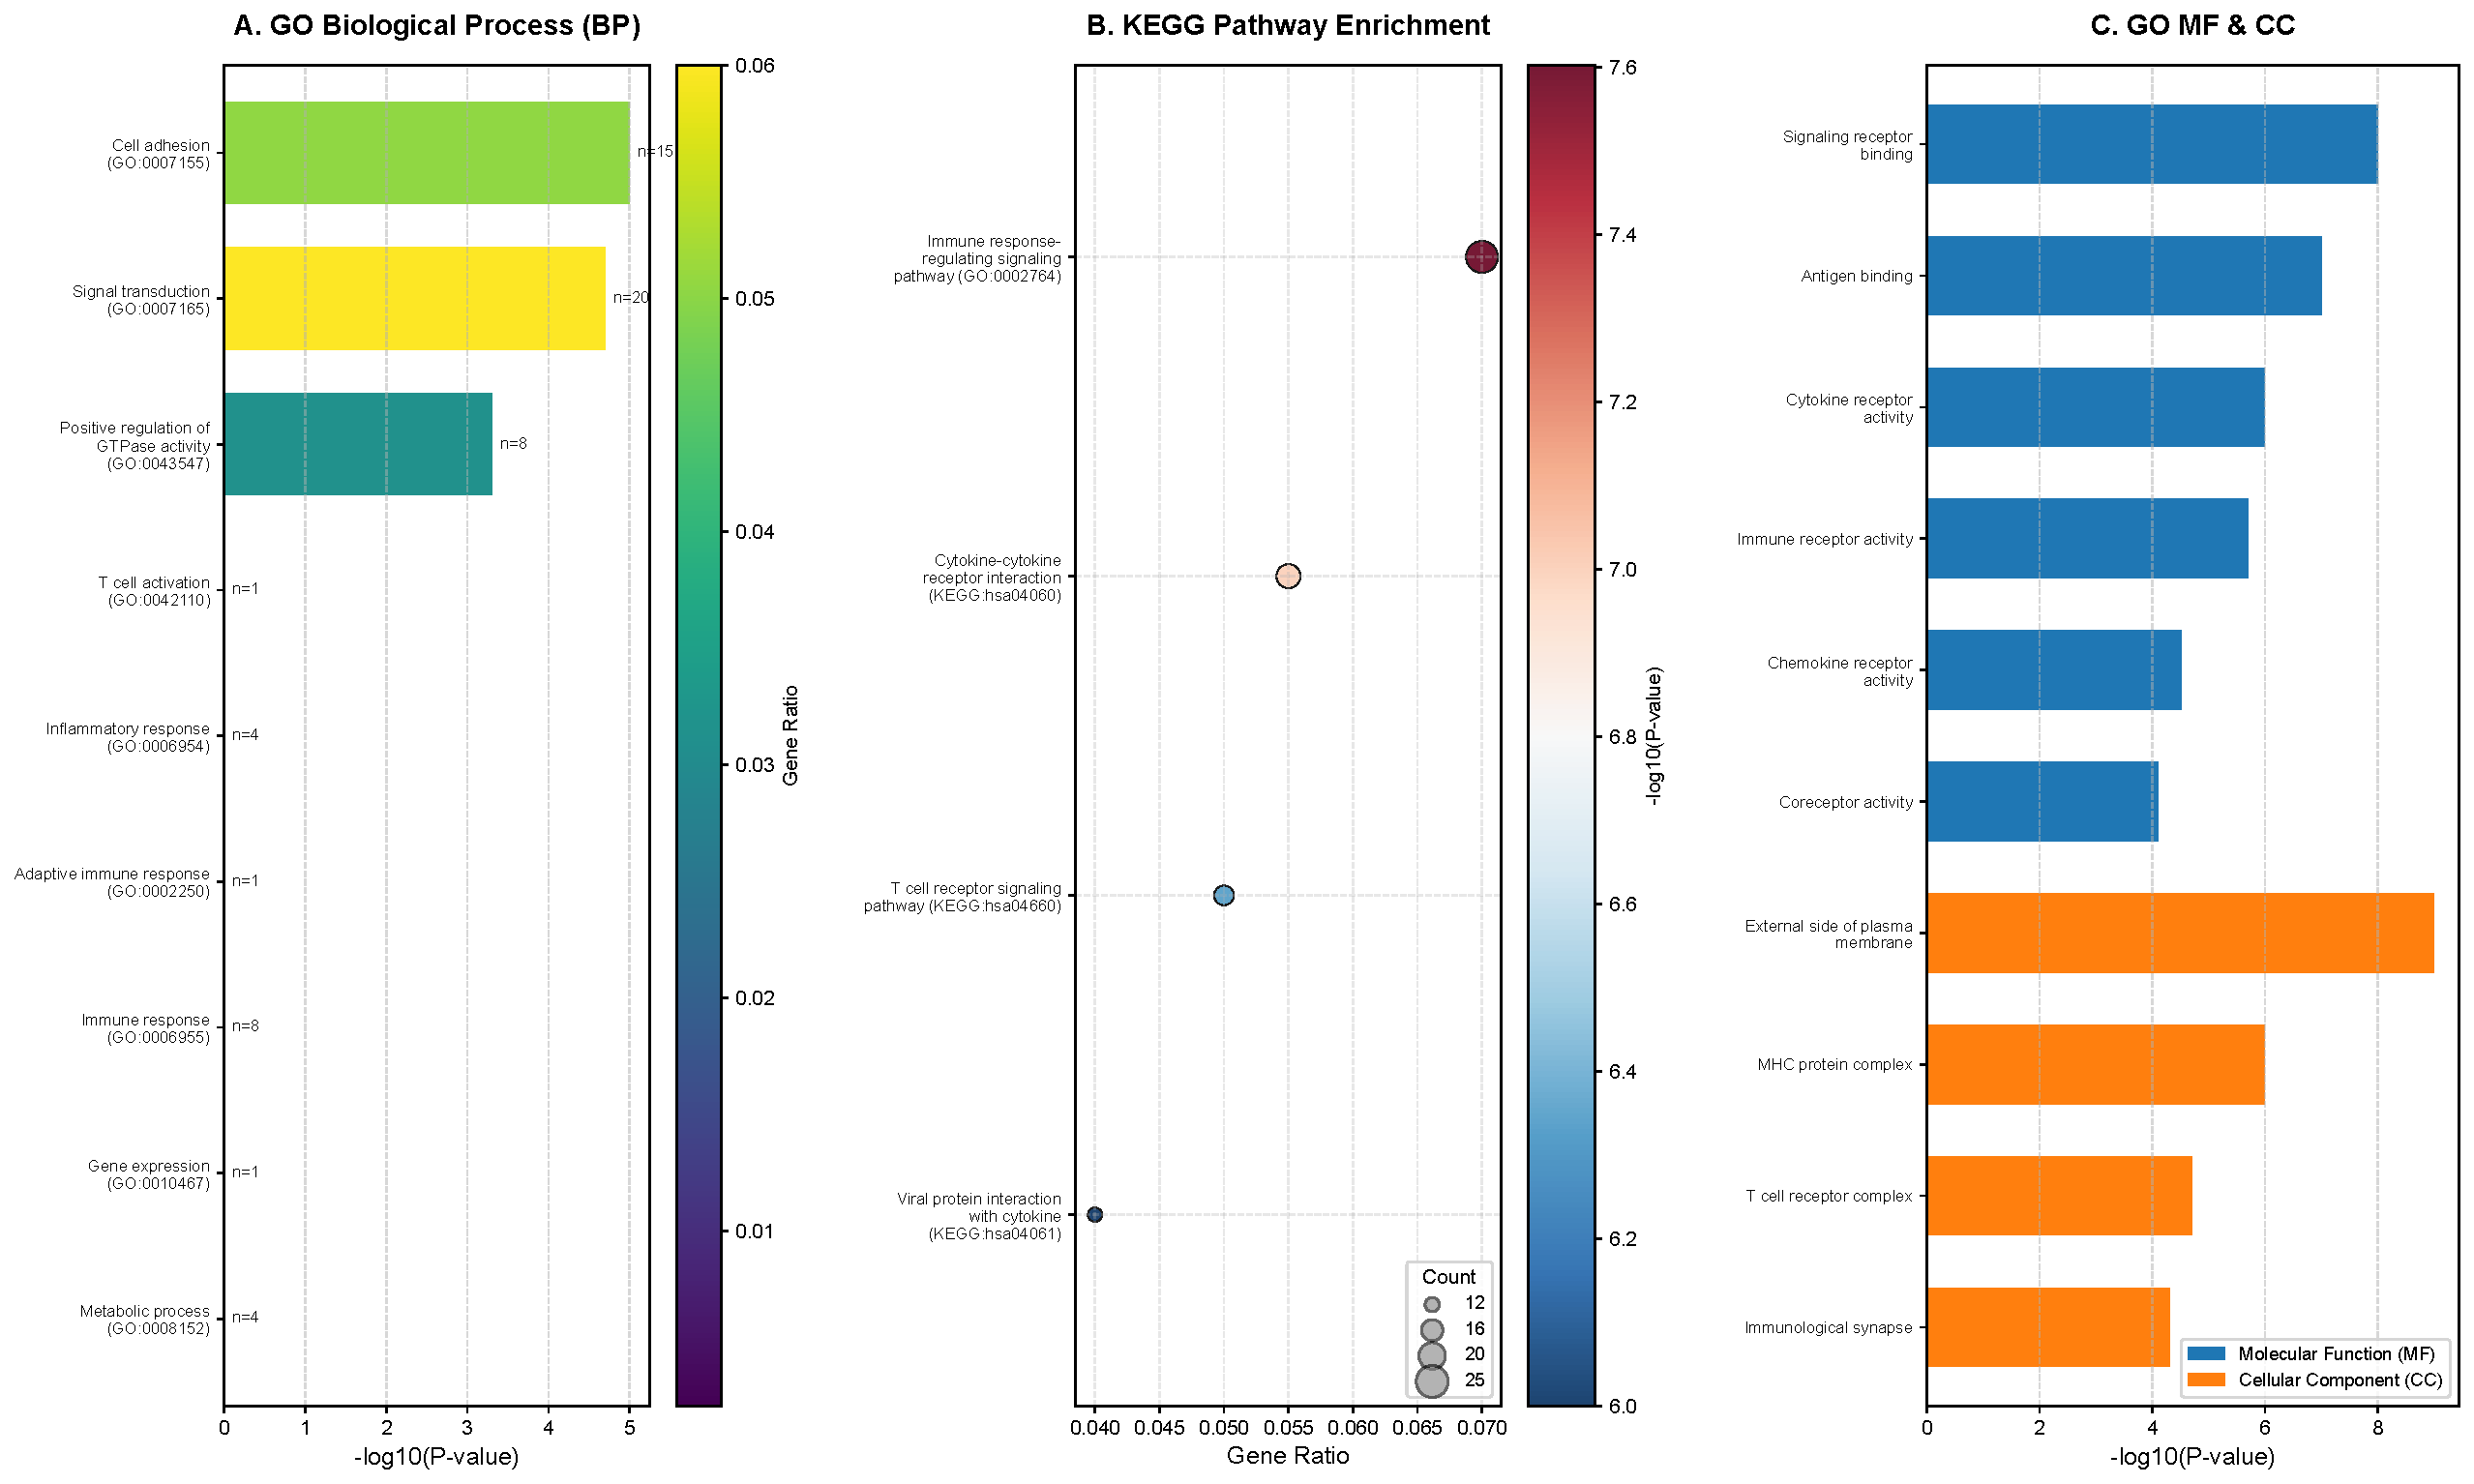
\includegraphics[width=0.95\textwidth]{FigureS3.pdf}
  \caption{\textbf{Functional enrichment analysis of model-associated genes.} (A) Gene Ontology (GO) biological process enrichment analysis. (B) KEGG pathway enrichment analysis. (C) Reactome pathway analysis results. (D) Protein-protein interaction (PPI) network of the top enriched genes.}
  \label{fig:S3}
\end{figure}

\begin{figure}[H]
  \centering
  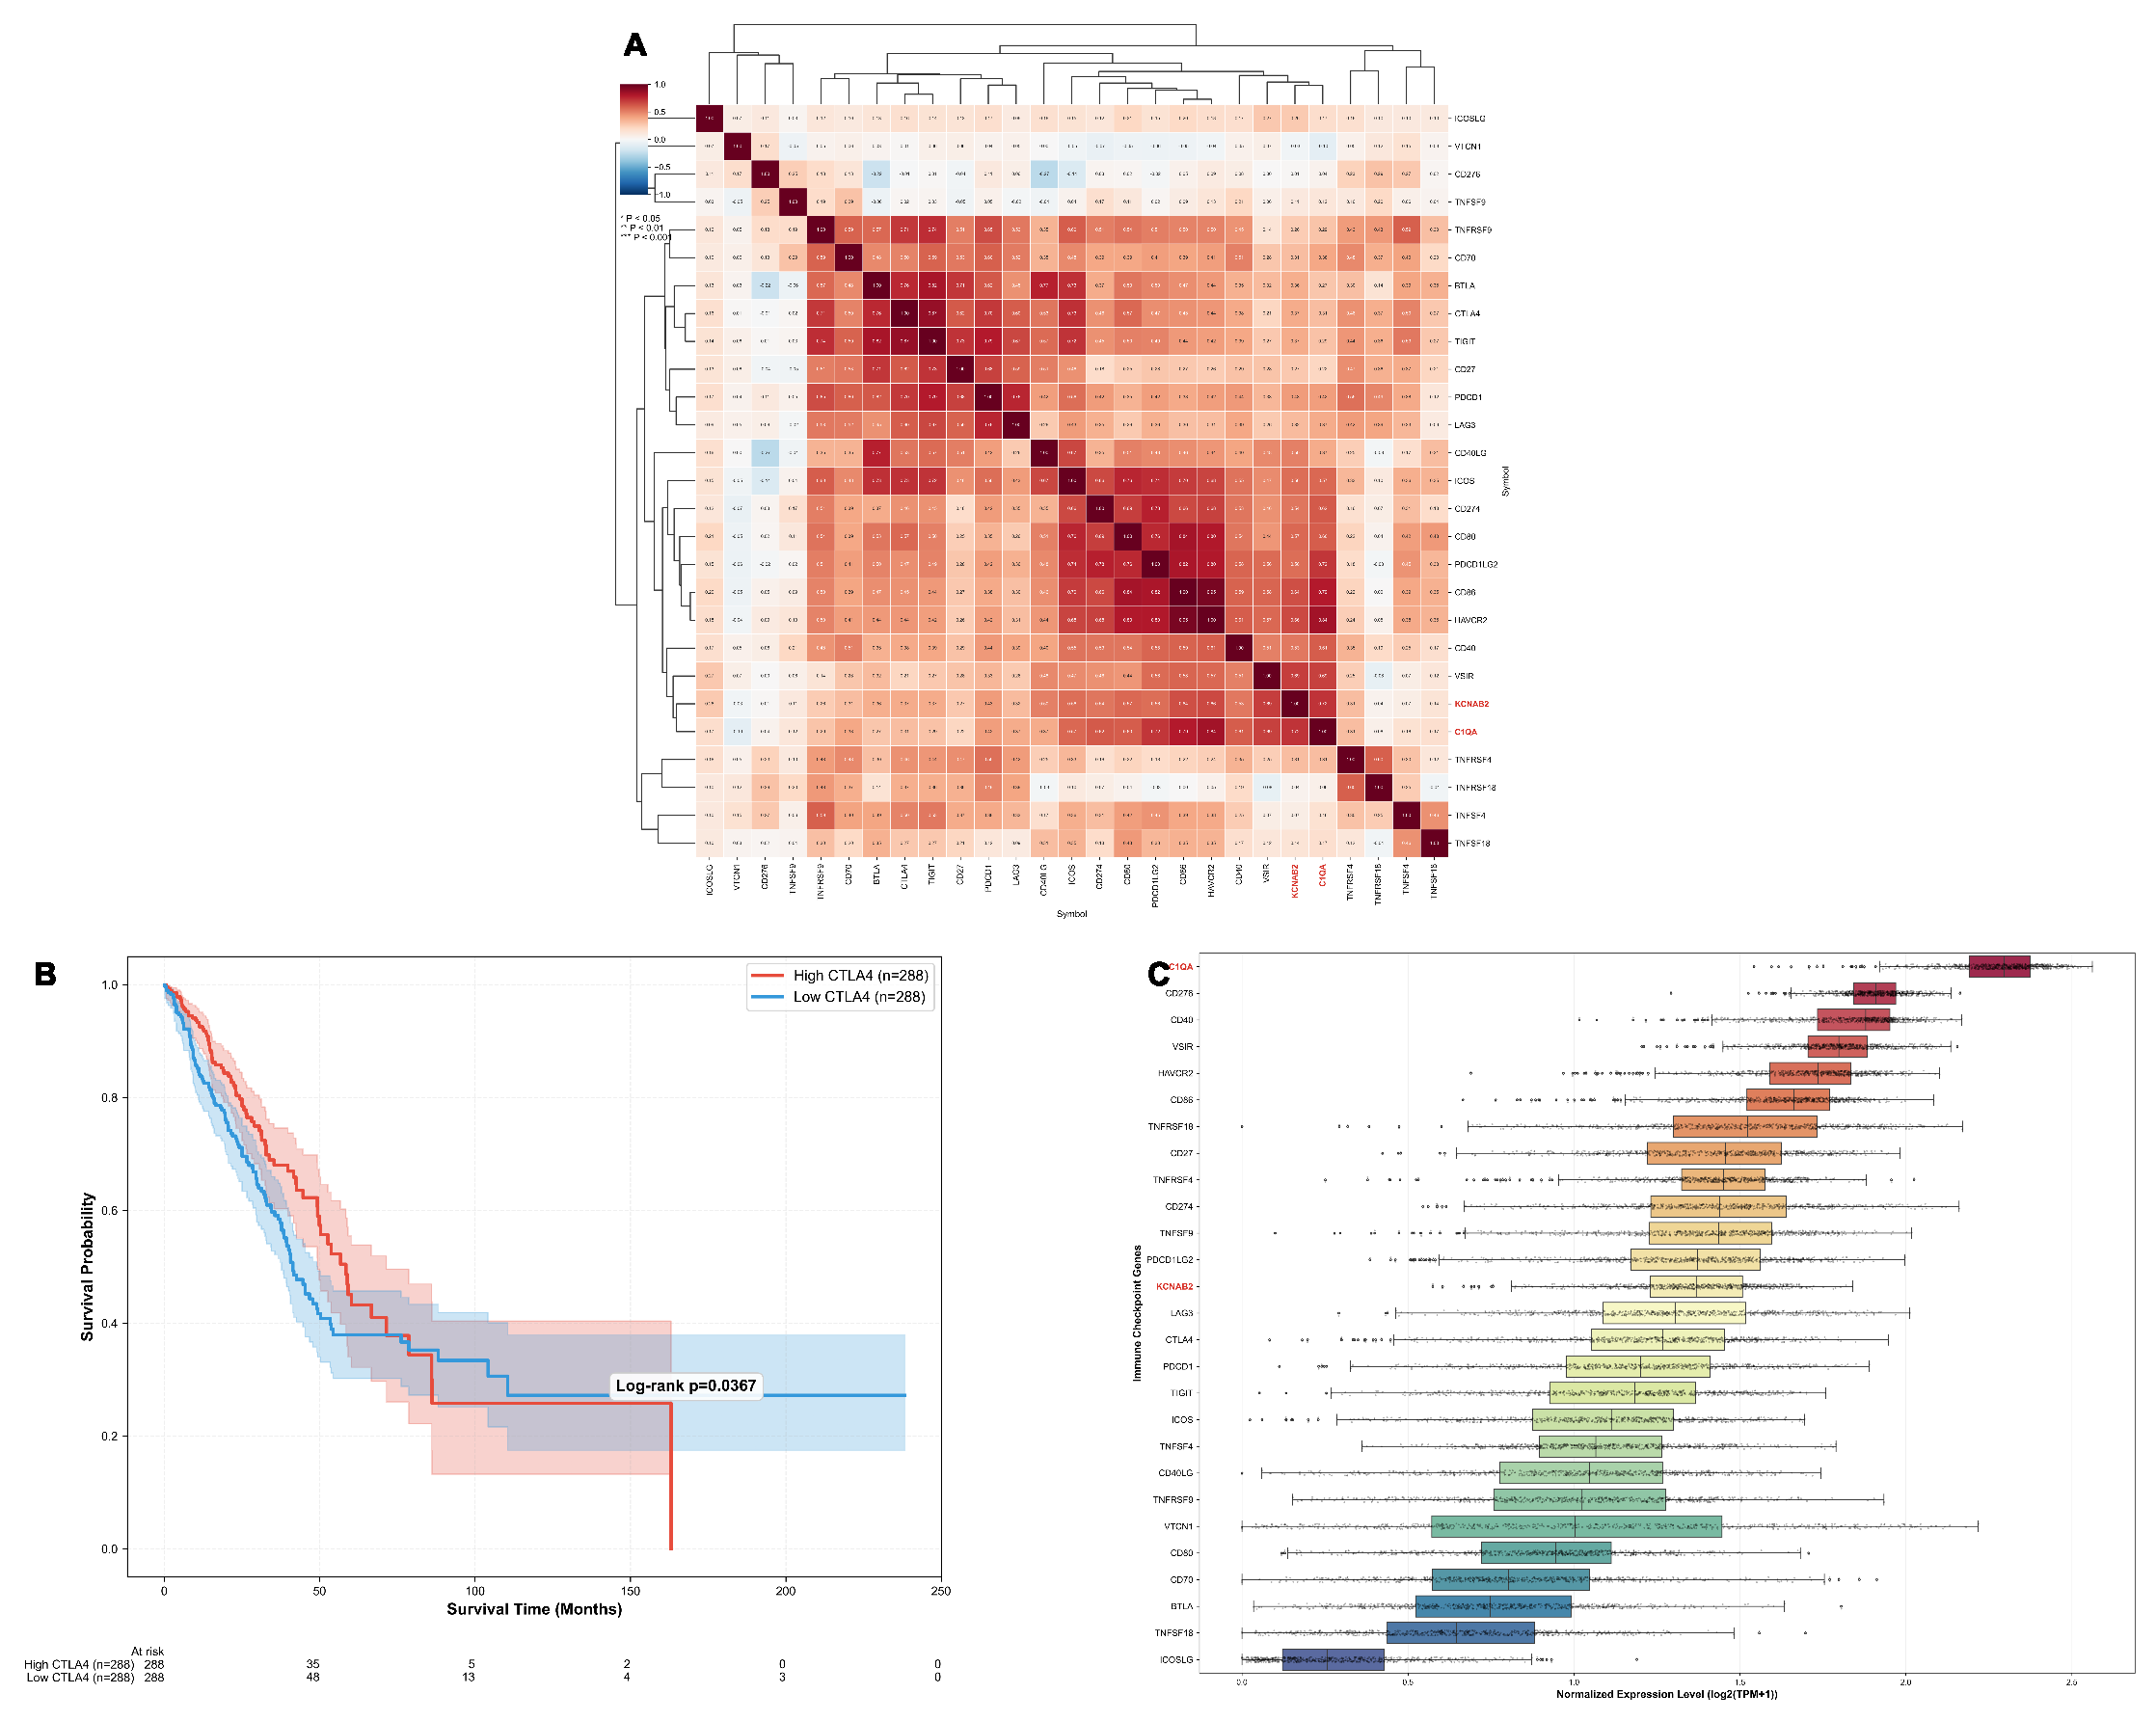
\includegraphics[width=0.95\textwidth]{FigureS4.pdf}
  \caption{\textbf{Spatial expression patterns of immune checkpoint molecules.} (A) Spatial expression plots of key immune checkpoints (e.g., \textit{PDCD1}, \textit{CD274}, \textit{CTLA4}). (B) Correlation matrix of checkpoint gene expression. (C) Spatial co-localization of checkpoints with immune cell markers. (D) Association between checkpoint expression and exploratory immune-context scores.}
  \label{fig:S4}
\end{figure}

\begin{figure}[H]
  \centering
  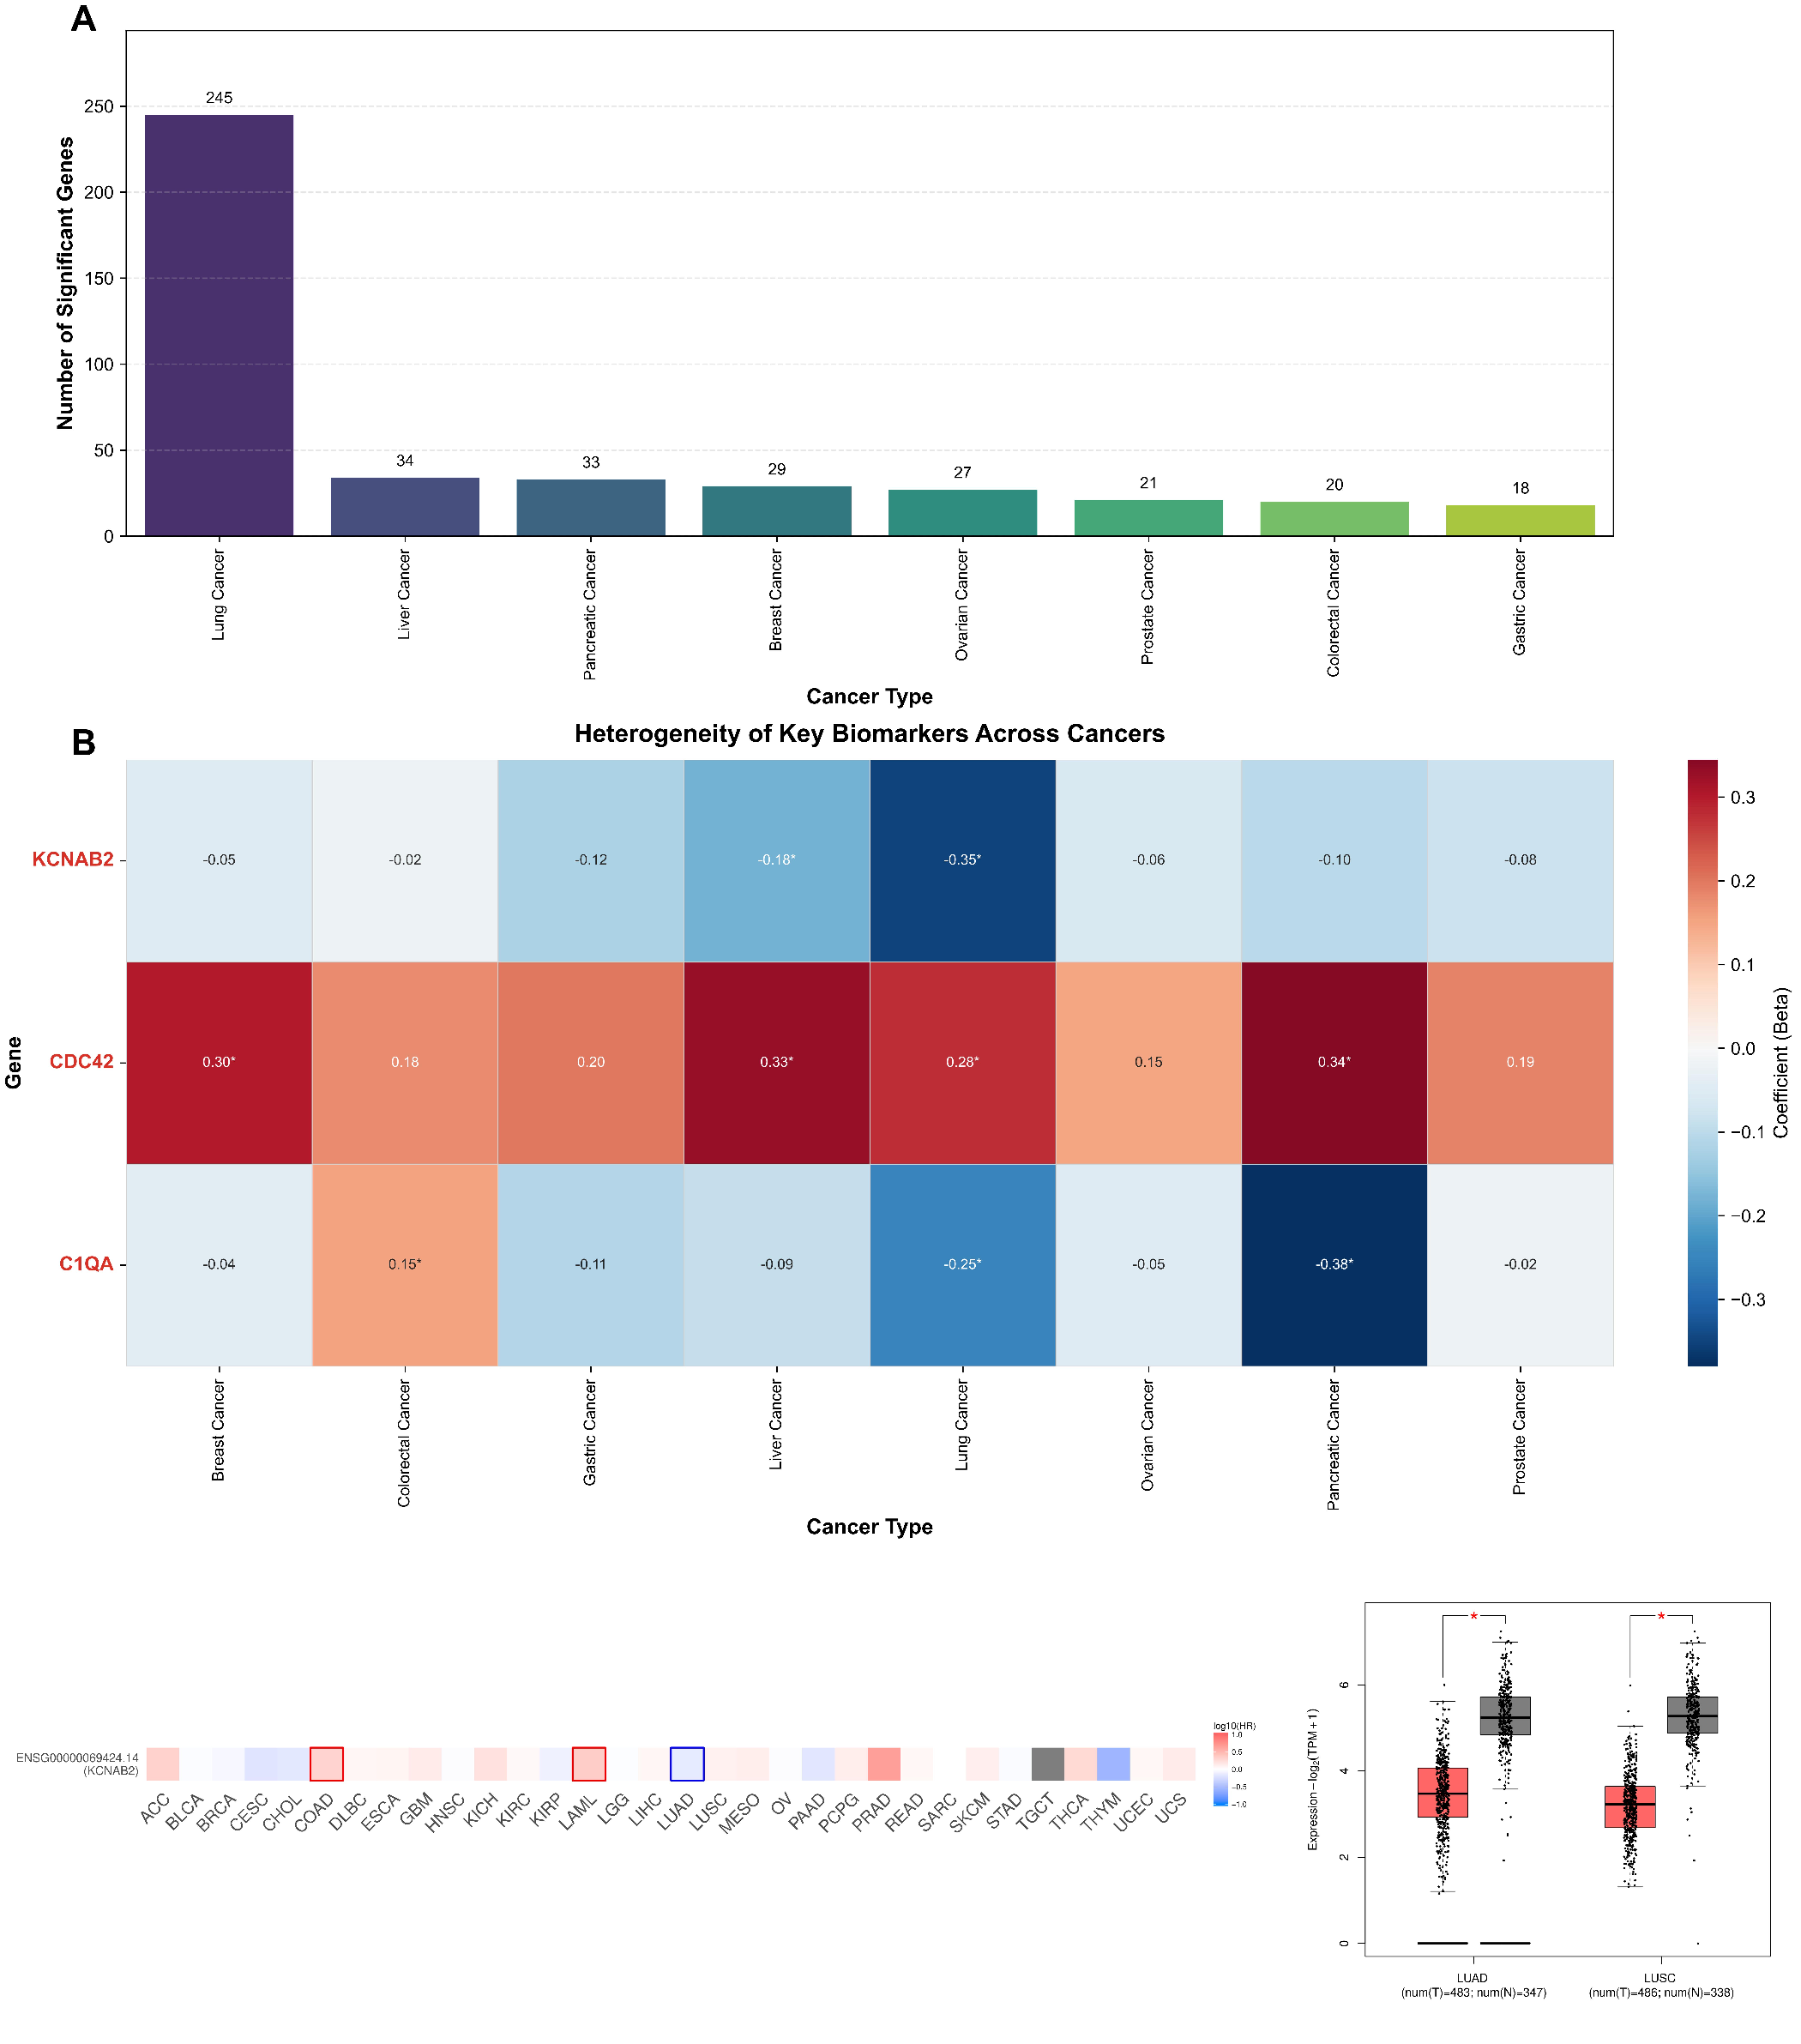
\includegraphics[width=0.95\textwidth]{FigureS5.pdf}
  \caption{\textbf{Pan-cancer exploratory traceability of core candidate genes.} (A) Statistical overview of significant genes identified across 33 cancer types in the exploratory screen. (B) Heatmap of prognostic coefficients (Beta) for five candidate genes (\textit{KCNAB2}, \textit{PLOD1}, \textit{CDC42}, \textit{TNF}, \textit{C1QA}) across 33 cancer types. (C) GEPIA-based Overall Survival Map for \textit{KCNAB2}, presented as an external context check rather than validation. (D) GEPIA Expression Boxplot for \textit{KCNAB2} in Lung Adenocarcinoma (LUAD) and Squamous Cell Carcinoma (LUSC).}
  \label{fig:S5}
\end{figure}

\begin{figure}[H]
  \centering
  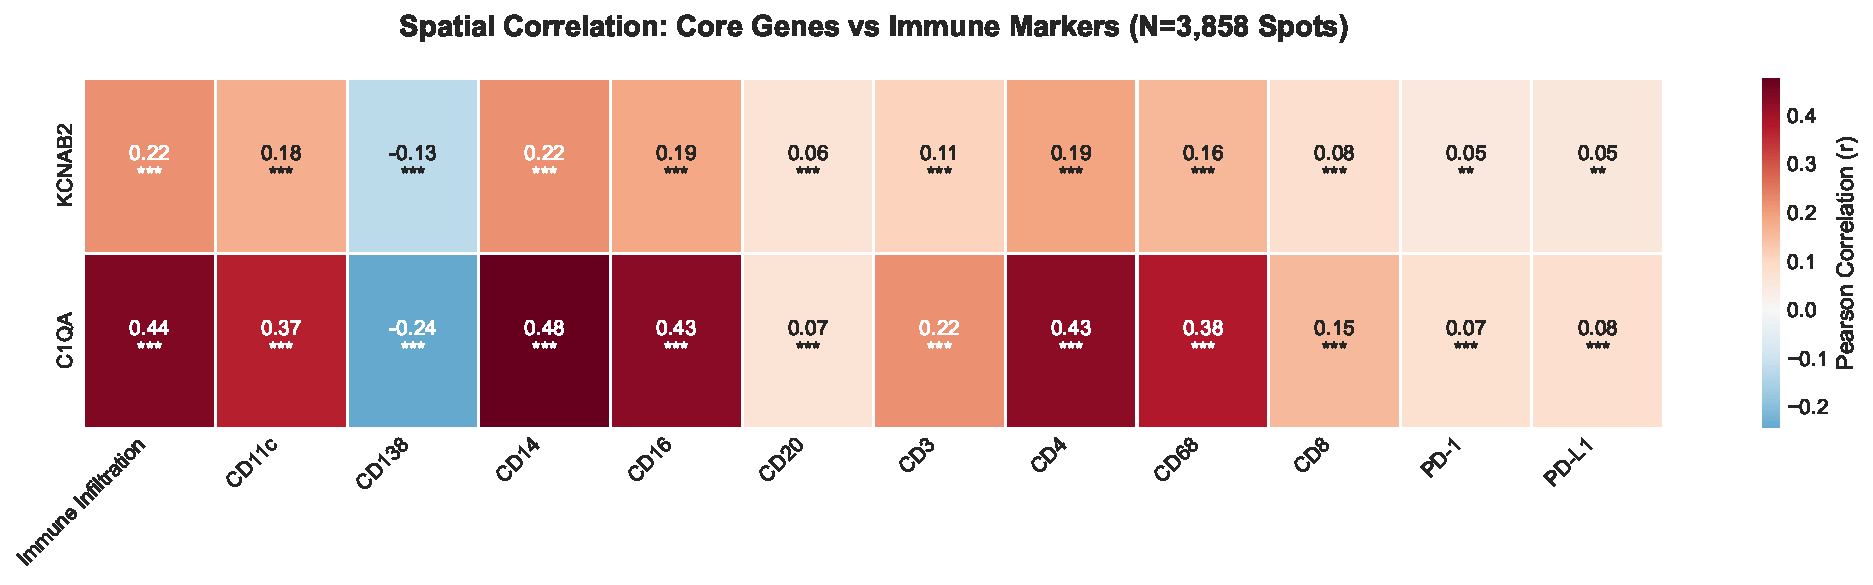
\includegraphics[width=0.95\textwidth]{FigureS6.pdf}
  \caption{\textbf{Correlation analysis between hub genes and immune-context estimates.} Clustered heatmap displaying Pearson correlation coefficients between hub genes (\textit{KCNAB2}, \textit{PLOD1}) and 23 immune-context estimates predicted by GigaTIME. Red indicates positive correlation; blue indicates negative correlation. * $P < 0.050$, ** $P < 0.010$, *** $P < 0.001$. CD138 is interpreted as plasma-cell context, not as a macrophage marker.}
  \label{fig:S6}
\end{figure}

\begin{figure}[H]
  \centering
  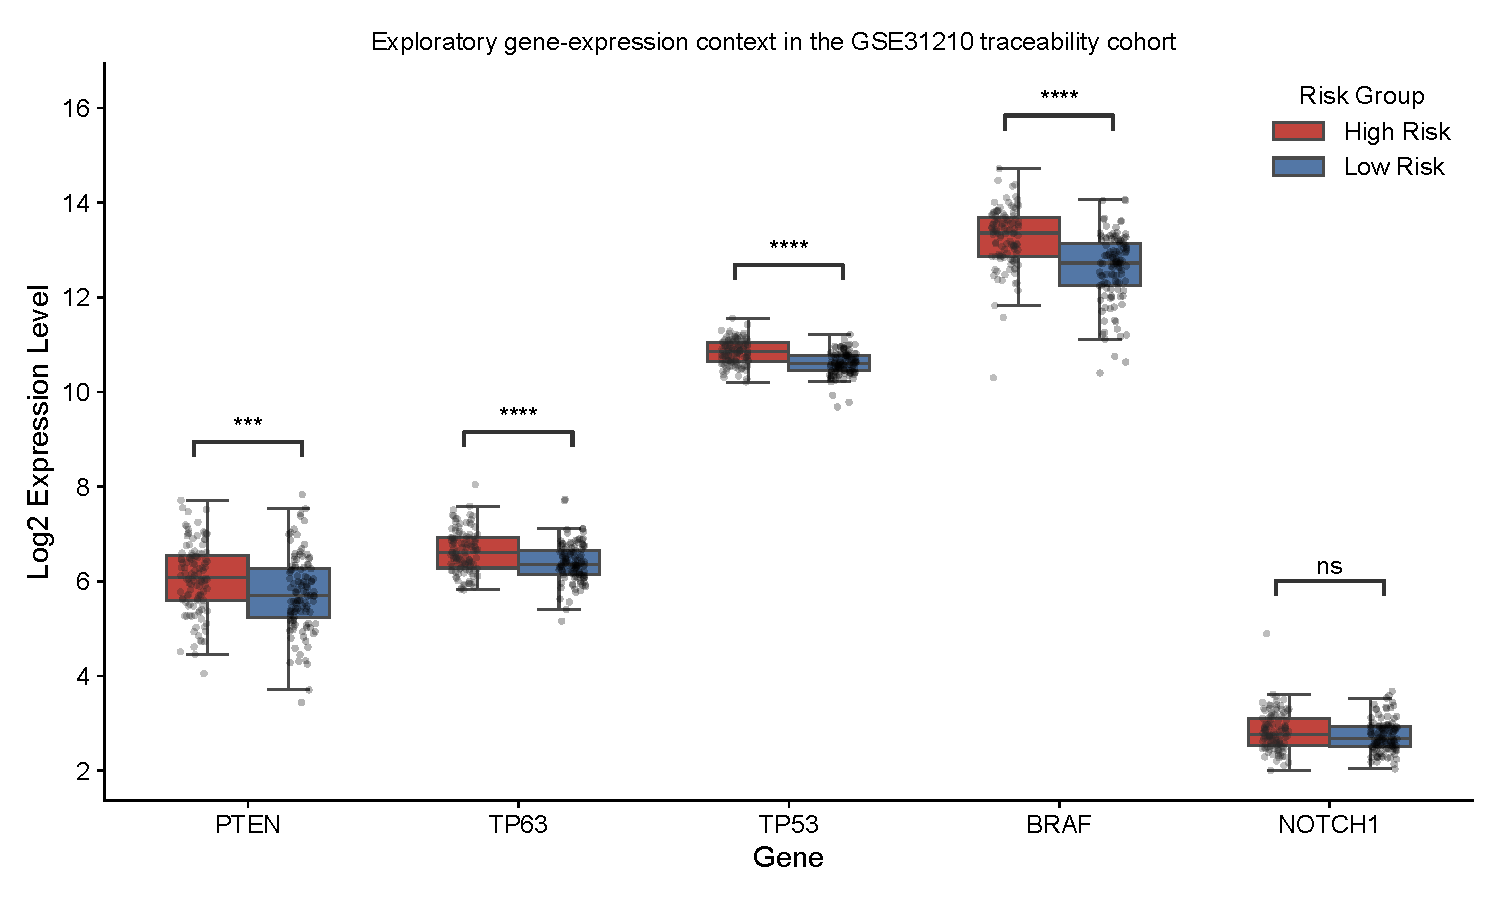
\includegraphics[width=0.95\textwidth]{FigureS7.pdf}
  \caption{\textbf{Expression of top model genes in the GSE31210 traceability cohort.} Boxplots showing the expression levels of the top contributing model features (including \textit{ACP5}, \textit{KCNAB2}, \textit{BOK}, \textit{ADAMTS1}, and \textit{CASP8}) in the GSE31210 high- and low-risk groups. These genes represent statistical contributors to the exploratory model, while \textit{KCNAB2} and \textit{C1QA} were further prioritized for follow-up based on selection stability and MR-based association. Statistical significance was assessed using the Mann-Whitney U test (* $P < 0.050$, ** $P < 0.010$, *** $P < 0.001$, **** $P < 0.000$).}
  \label{fig:S7}
\end{figure}

\begin{figure}[H]
  \centering
  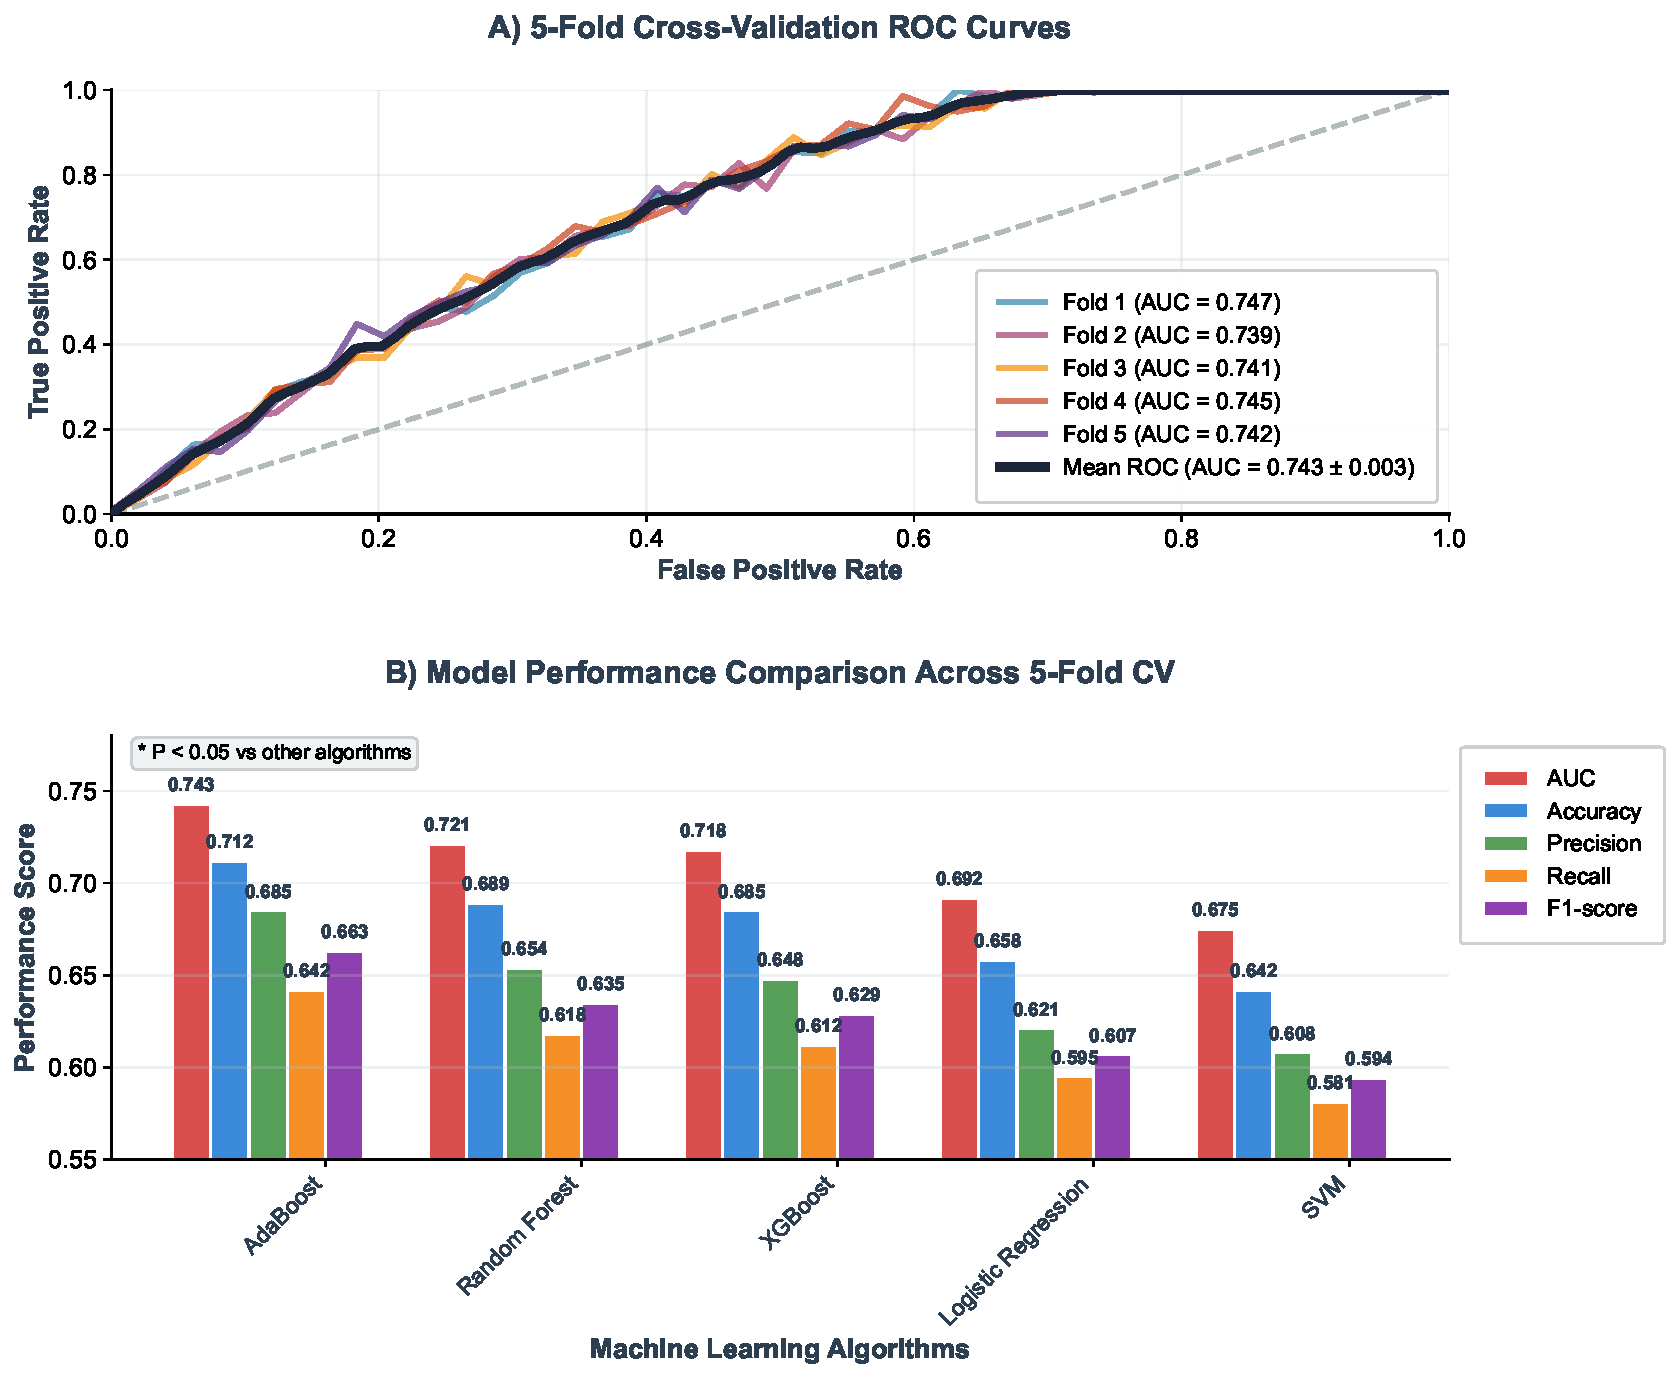
\includegraphics[width=0.95\textwidth]{FigureS8.pdf}
  \caption{\textbf{5-fold cross-validation performance evaluation and model comparison.} (A) ROC curves from each of the 5 cross-validation folds. The mean AUC across all folds was 0.743 $\pm$ 0.028, indicating internally reproducible but retrospective discrimination. (B) Performance comparison bar chart showing AUC, Accuracy, Precision, Recall, and F1-score across different machine learning algorithms (AdaBoost, Random Forest, XGBoost, Logistic Regression, SVM). Algorithm rankings varied by metric; no single model is interpreted as clinically superior. Error bars represent standard deviation across the 5 CV folds.}
  \label{fig:S8}
\end{figure}

\begin{figure}[H]
  \centering
  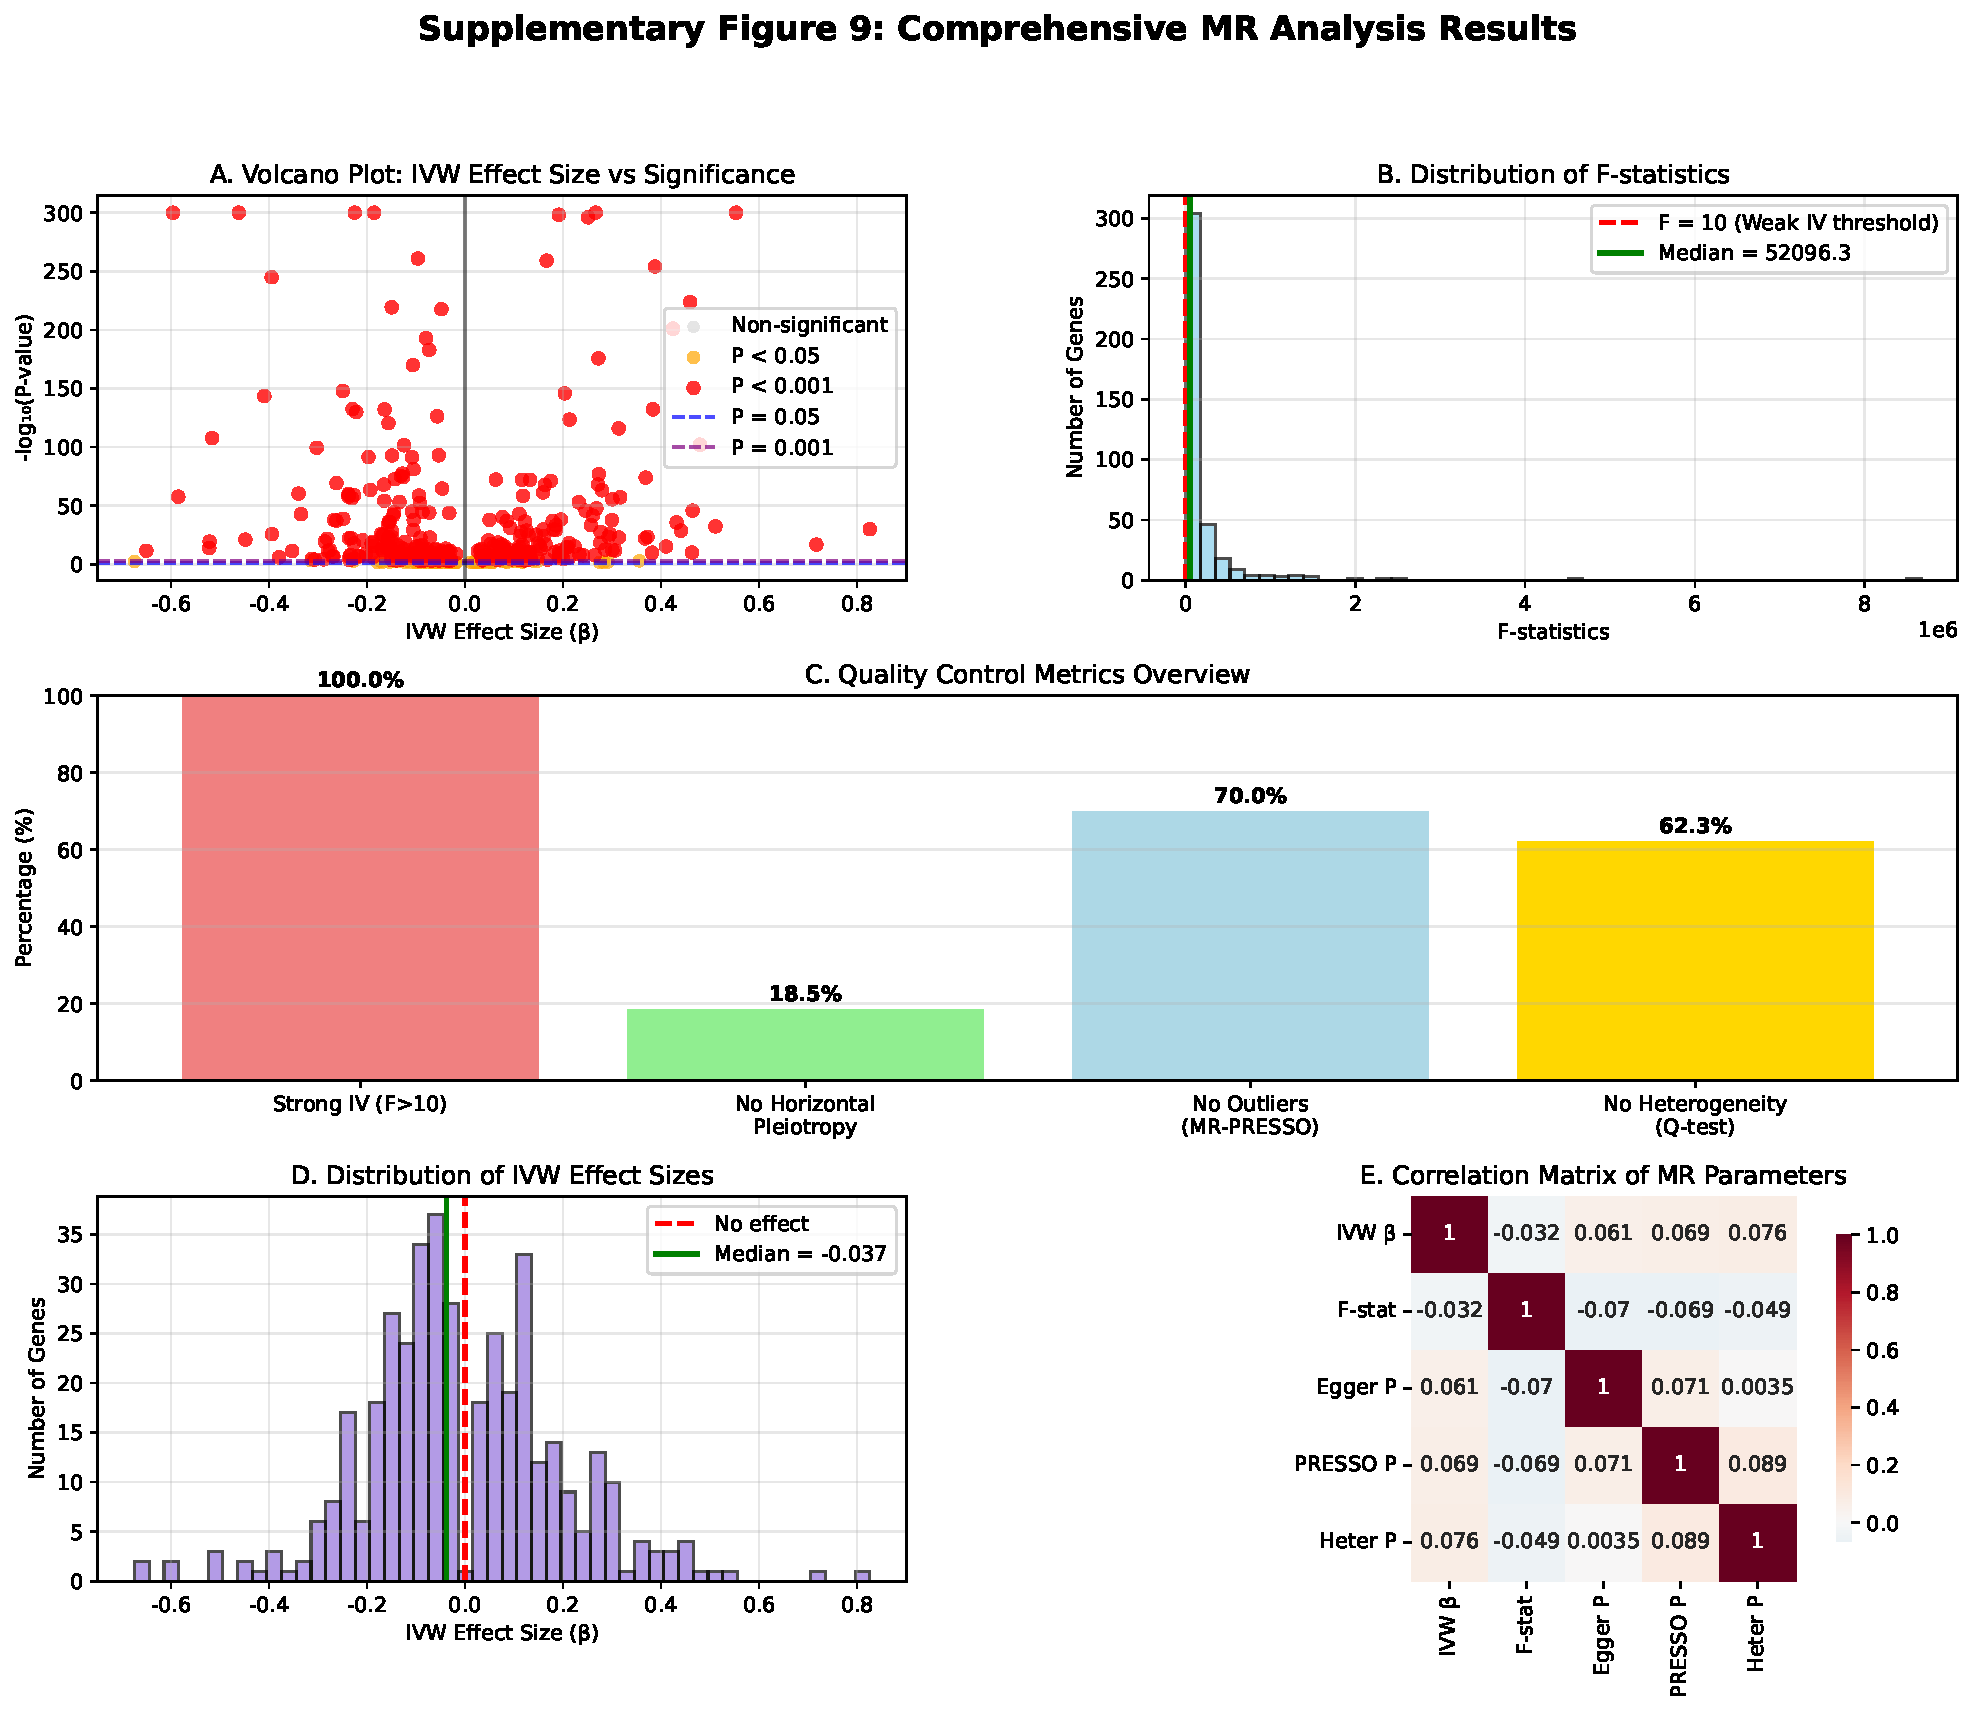
\includegraphics[width=0.95\textwidth]{FigureS9.pdf}
  \caption{\textbf{Mendelian-randomization leave-one-out sensitivity analysis.} Leave-one-out plots for prioritized genes (including \textit{KCNAB2}, \textit{C1QA}, and \textit{ACP5}), showing whether the MR estimate is dominated by any single instrumental variable (SNP). These analyses support gene prioritization under instrumental-variable assumptions but do not prove mechanism.}
  \label{fig:S9}
\end{figure}

\begin{figure}[H]
  \centering
  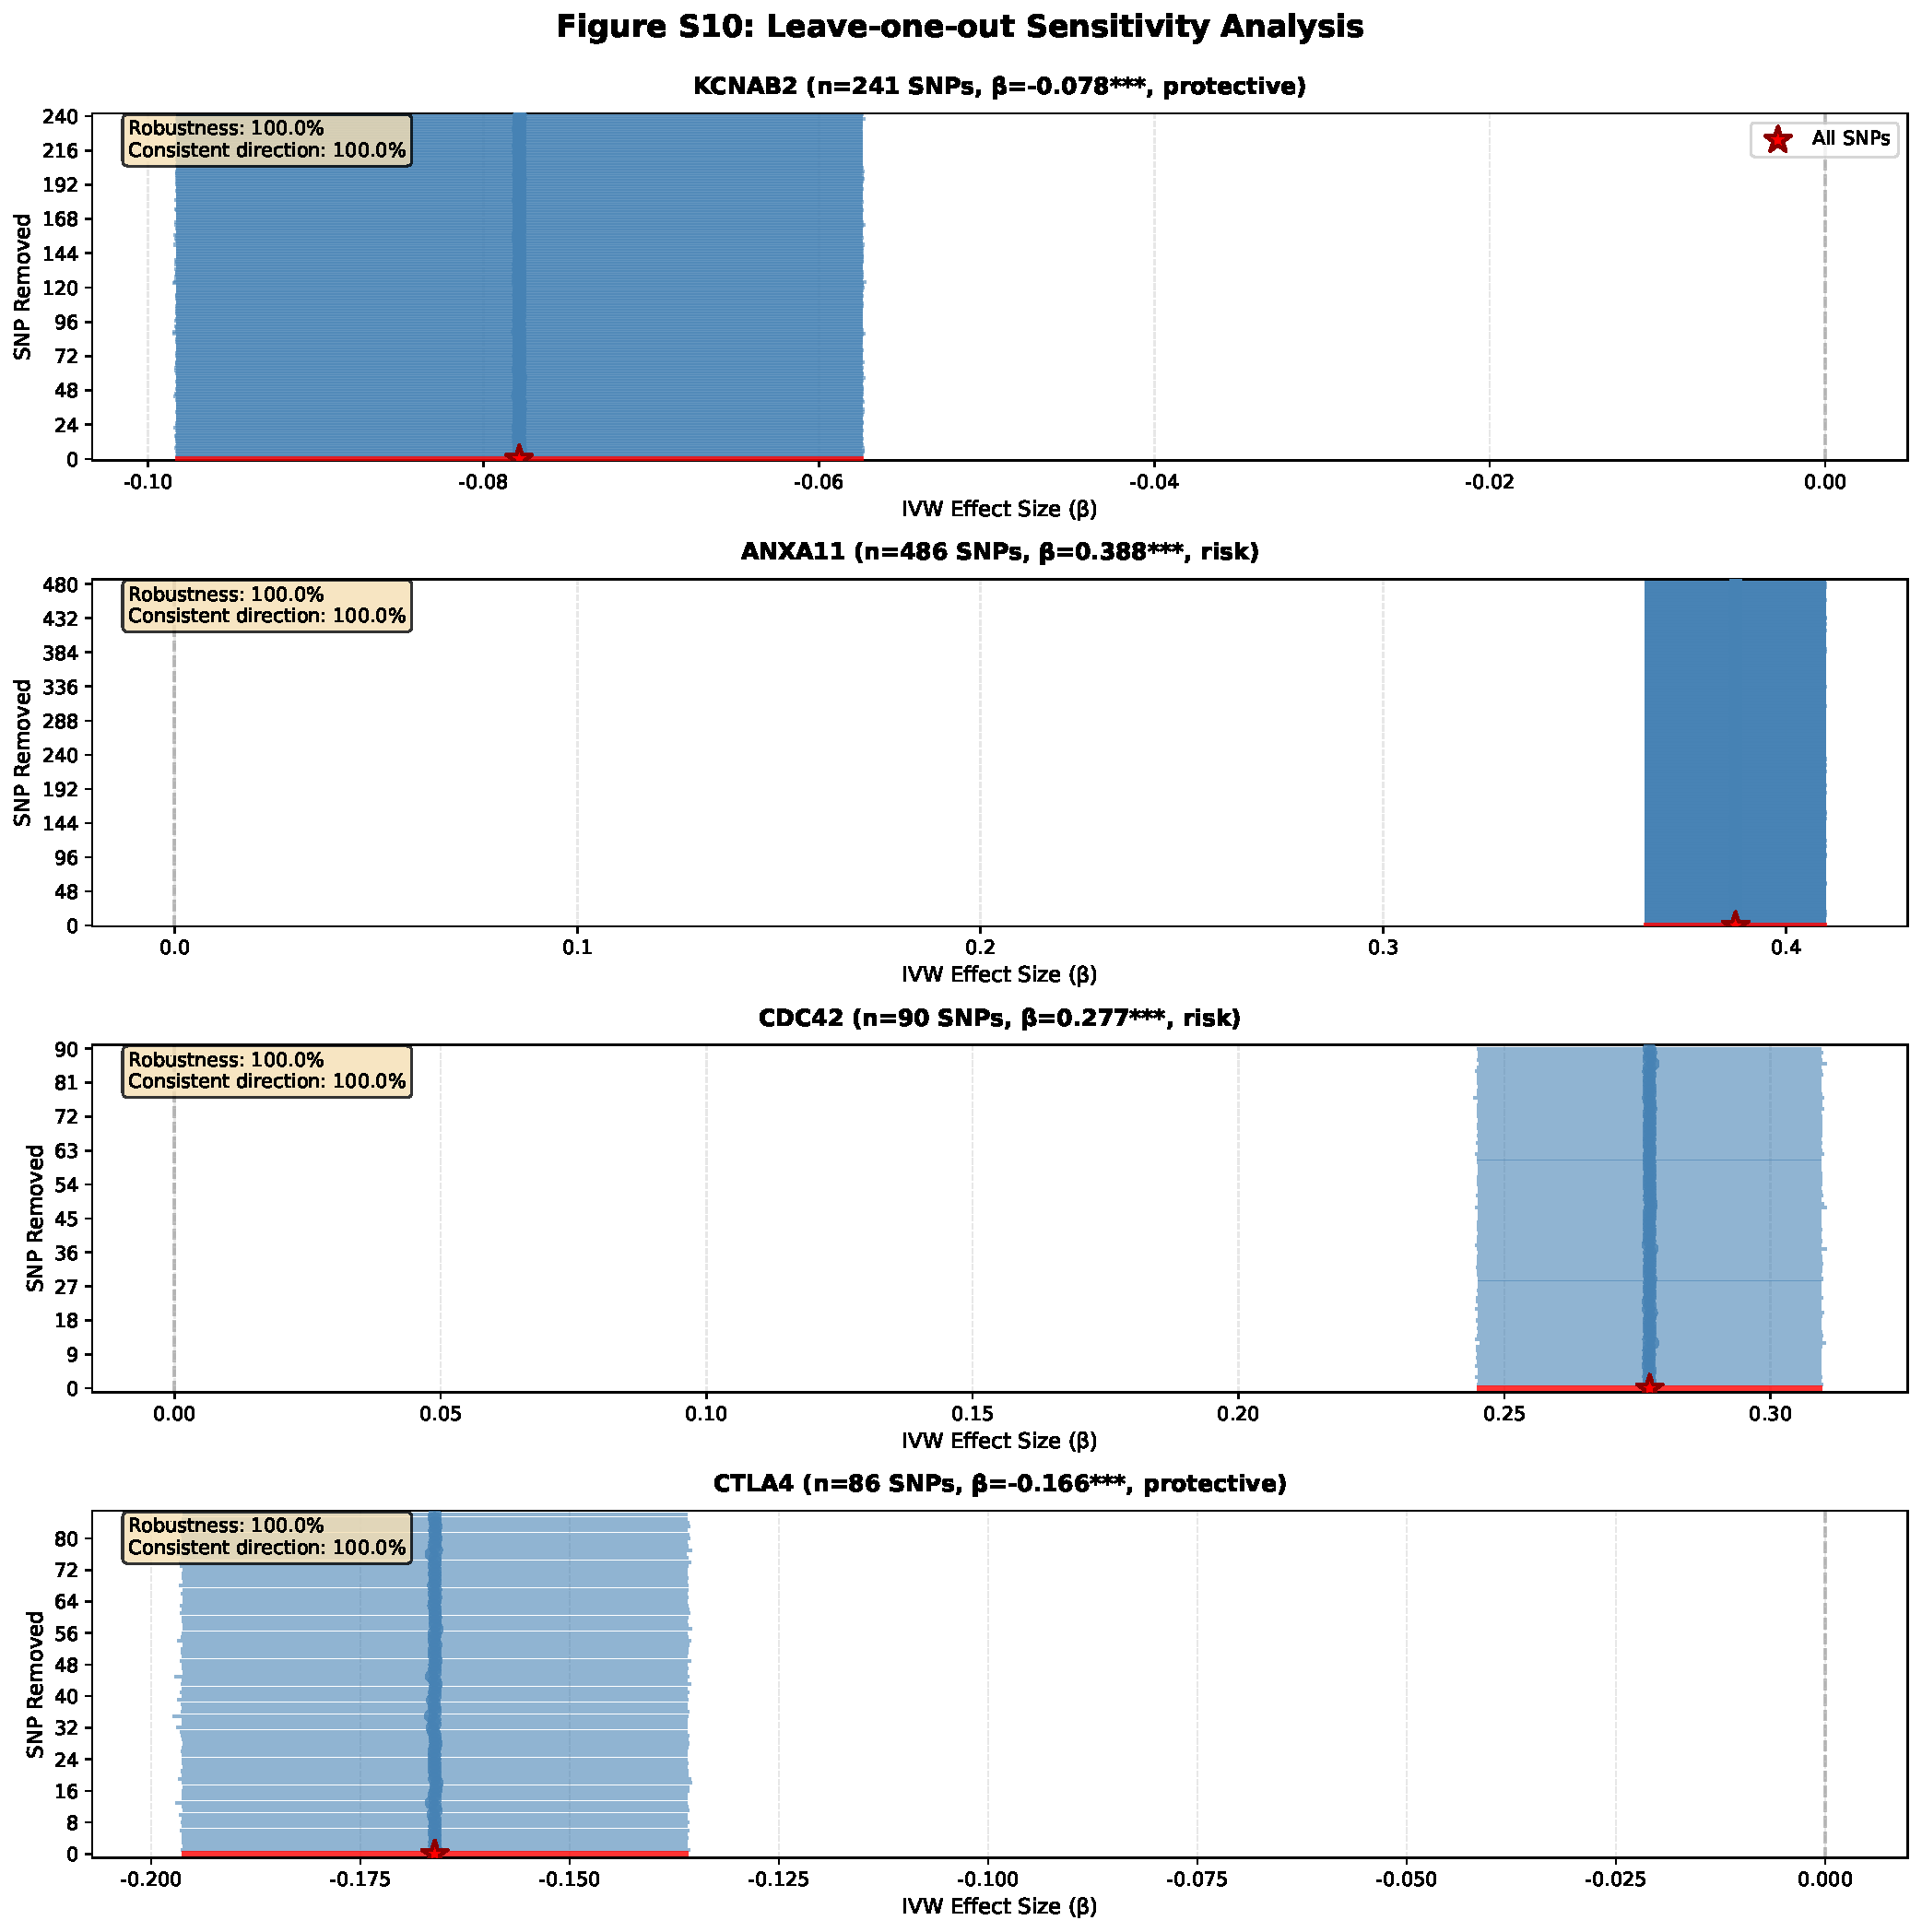
\includegraphics[width=0.95\textwidth]{FigureS10.pdf}
  \caption{\textbf{Leave-one-out sensitivity analysis for MR-prioritized genes.} Each point represents the recalculated inverse variance weighted (IVW) estimate after systematically removing one SNP at a time. The red star indicates the original estimate using all SNPs. Error bars represent 95\% confidence intervals. The dashed vertical line indicates the null effect ($\beta$ = 0). Stable direction across leave-one-out analyses is interpreted as support for prioritization, not as definitive causal proof.}
  \label{fig:S10}
\end{figure}

\begin{figure}[H]
  \centering
  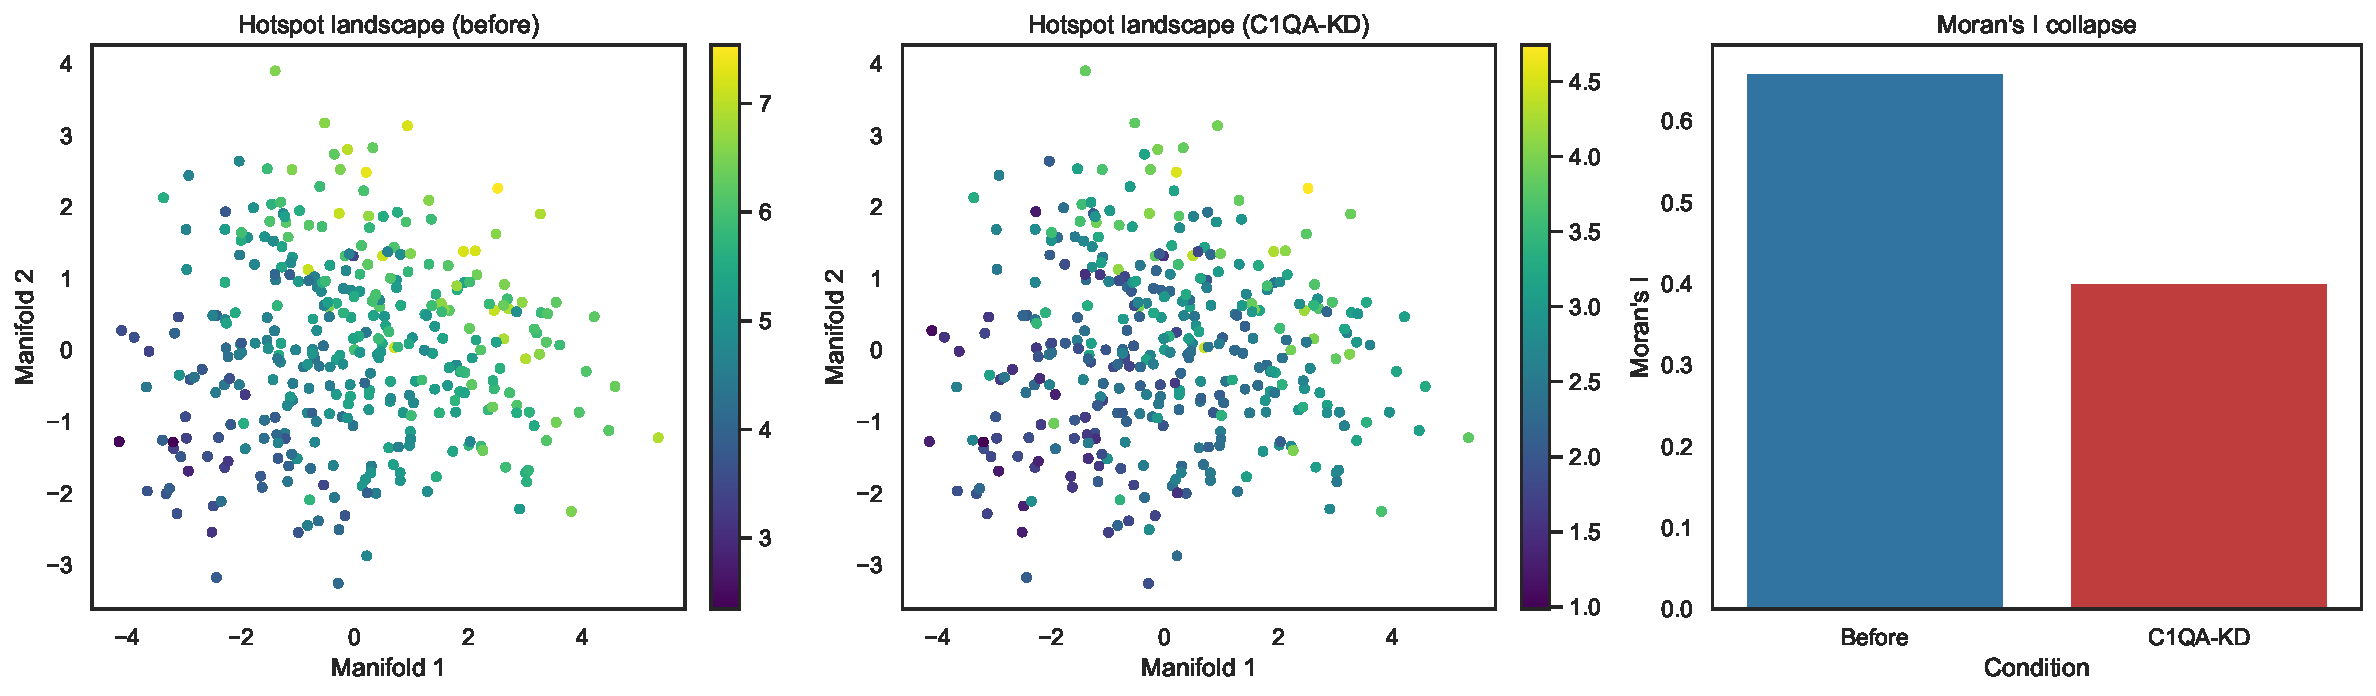
\includegraphics[width=0.95\textwidth]{virtual_perturbation/FigureY_hotspot_collapse.pdf}
  \caption{\textbf{Counterfactual C1QA scoring sensitivity of spatial summaries.} Transcriptomic manifold maps before and after computational C1QA attenuation show reduced high-C1Q score regions. The paired Moran's I summary shows reduced spatial autocorrelation after score recomputation, supporting score dependency rather than experimental perturbation or causal proof.}
  \label{fig:S11}
\end{figure}

\begin{figure}[H]
  \centering
  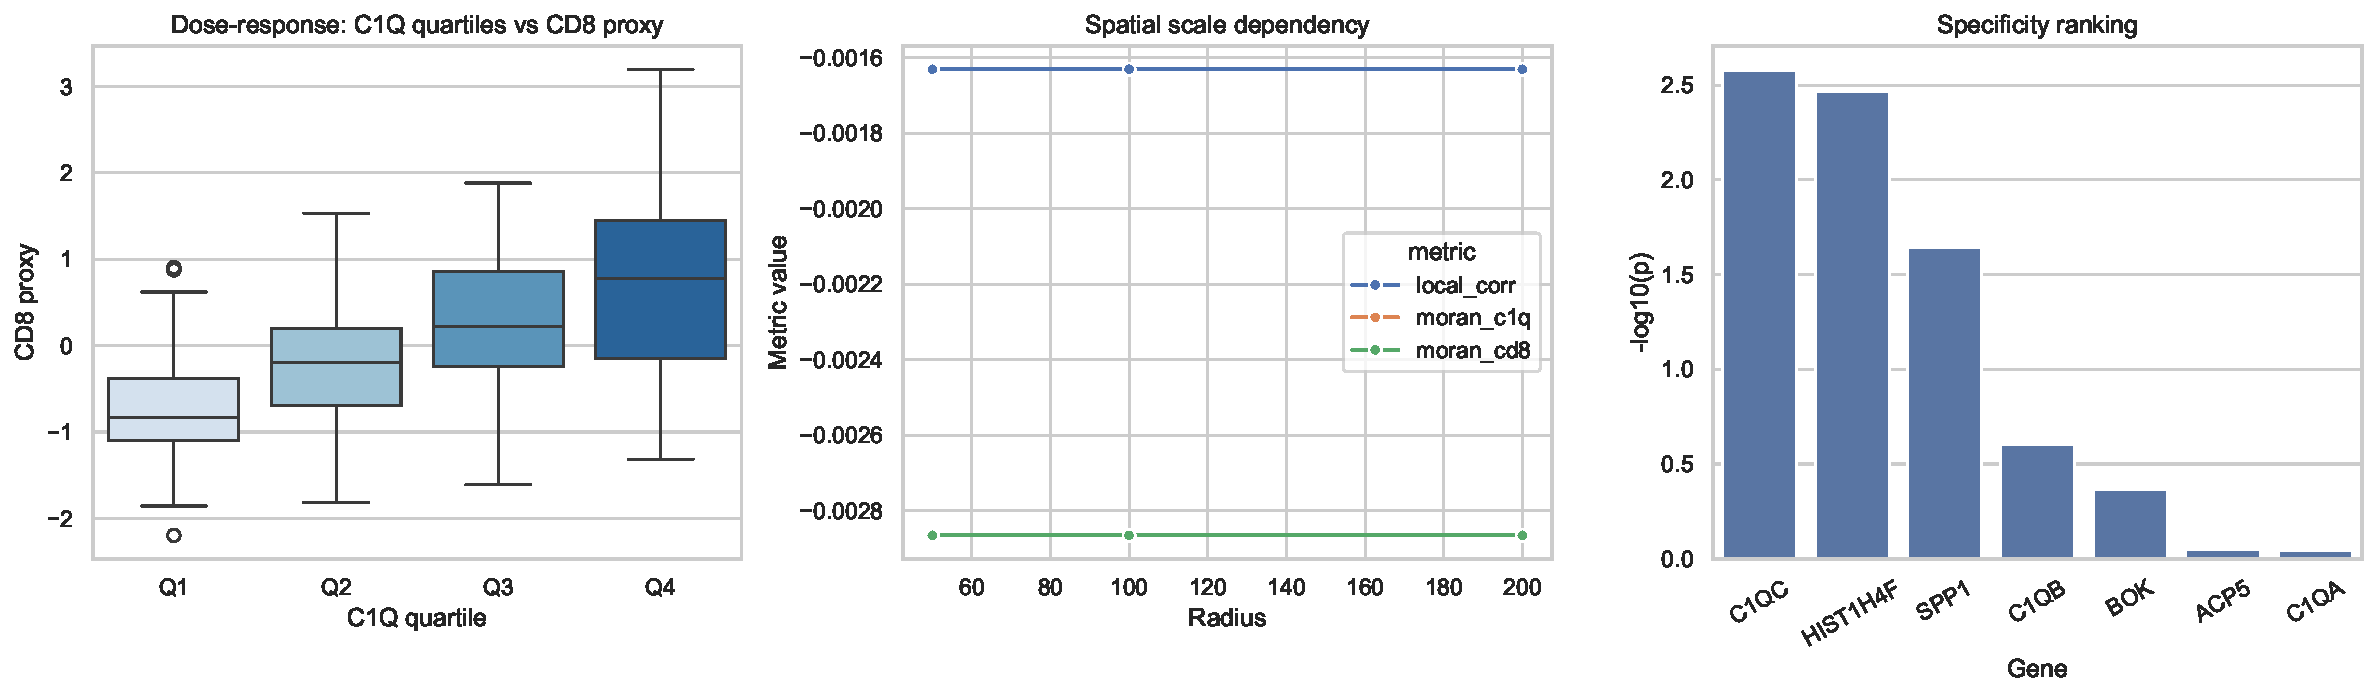
\includegraphics[width=0.95\textwidth]{virtual_perturbation/FigureS12_mechanism_modules.pdf}
  \caption{\textbf{Sensitivity modules for C1Q-context interpretation.} Left: dose-response relationship between C1Q quartiles and CD8 proxy activity. Middle: spatial scale dependency of local coupling and spatial autocorrelation across 50/100/200 radii. Right: specificity ranking of C1Q-axis genes versus non-C1Q controls based on survival-linked statistical signal.}
  \label{fig:S12}
\end{figure}

\newpage

\section{Supplementary Tables}

\clearpage

\begin{landscape}
  \pagestyle{empty}
  \newgeometry{left=1cm, right=1cm, top=2cm, bottom=2cm}
  {
    \tiny
    \setlength{\tabcolsep}{4pt}
    \renewcommand{\arraystretch}{1.3}
    \setlength\LTleft{0pt}
    \setlength\LTright{\fill}
    \setcounter{table}{0}
    \renewcommand{\thetable}{S1a}

    \begin{longtable}{l >{\raggedright\arraybackslash}p{10cm} *{5}{c}}
      \caption{Model Performance on Training Set} \label{tab:Table_S1a}                                                                                               \\
      \toprule
      \textbf{Model}      & \textbf{Hyperparameters}                                       & \textbf{Acc} & \textbf{Prec} & \textbf{Rec} & \textbf{F1} & \textbf{AUC} \\
      \midrule
      \endfirsthead
      \caption[]{\textbf{Table S1a (Continued)}}                                                                                                                      \\
      \toprule
      \textbf{Model}      & \textbf{Hyperparameters}                                       & \textbf{Acc} & \textbf{Prec} & \textbf{Rec} & \textbf{F1} & \textbf{AUC} \\
      \midrule
      \endhead
      Logistic Regression & \seqsplit{C=1.0, solver=lbfgs, max\_iter=1000}                 & 0.865        & 0.842         & 0.816        & 0.829       & 0.929        \\
      Decision Tree       & \seqsplit{criterion=gini, max\_depth=None, splitter=best}      & 1.000        & 1.000         & 1.000        & 1.000       & 1.000        \\
      Random Forest       & \seqsplit{n\_estimators=200, criterion=gini, max\_depth=None}  & 1.000        & 1.000         & 1.000        & 1.000       & 1.000        \\
      Gradient Boosting   & \seqsplit{n\_estimators=100, learning\_rate=0.1, max\_depth=3} & 1.000        & 1.000         & 1.000        & 1.000       & 1.000        \\
      AdaBoost            & \seqsplit{n\_estimators=100, learning\_rate=1.0}               & 1.000        & 1.000         & 1.000        & 1.000       & 1.000        \\
      Soft Voting         & \seqsplit{AdaBoost, RF, LogReg (Ensemble)}                     & 0.925        & 0.891         & 0.864        & 0.877       & 0.962        \\
      XGBoost             & \seqsplit{n\_estimators=100, max\_depth=3, learning\_rate=0.1} & 1.000        & 1.000         & 1.000        & 1.000       & 1.000        \\
      SVM                 & \seqsplit{C=1.0, kernel=rbf, gamma=scale}                      & 0.853        & 0.869         & 0.745        & 0.802       & 0.958        \\
      K-Nearest Neighbors & \seqsplit{n\_neighbors=5, weights=uniform, algorithm=auto}     & 0.771        & 0.678         & 0.816        & 0.741       & 0.846        \\
      Naive Bayes         & \seqsplit{var\_smoothing=1e-09}                                & 0.702        & 0.602         & 0.755        & 0.670       & 0.788        \\
      \bottomrule
    \end{longtable}

    \vspace{1cm}
    \addtocounter{table}{-1}
    \renewcommand{\thetable}{S1b}

    \begin{longtable}{l *{5}{c} *{5}{c} c}
      \caption{Model Performance on Validation, Test, and External Sets} \label{tab:Table_S1b}                                                                                                                     \\
      \toprule
                          & \multicolumn{5}{c}{\textbf{Validation Set}} & \multicolumn{5}{c}{\textbf{Test Set}} & \textbf{Ext.}                                                                                    \\
      \cmidrule(lr){2-6} \cmidrule(lr){7-11} \cmidrule(lr){12-12}
      \textbf{Model}      & Acc                                         & Prec                                  & Rec            & F1             & AUC            & Acc   & Prec  & Rec   & F1    & AUC   & AUC   \\
      \midrule
      \endfirsthead
      \caption[]{\textbf{Table S1b (Continued)}}                                                                                                                                                                   \\
      \toprule
                          & \multicolumn{5}{c}{\textbf{Validation Set}} & \multicolumn{5}{c}{\textbf{Test Set}} & \textbf{Ext.}                                                                                    \\
      \cmidrule(lr){2-6} \cmidrule(lr){7-11} \cmidrule(lr){12-12}
      \textbf{Model}      & Acc                                         & Prec                                  & Rec            & F1             & AUC            & Acc   & Prec  & Rec   & F1    & AUC   & AUC   \\
      \midrule
      \endhead
      Logistic Regression & 0.531$\pm$0.08                              & 0.415$\pm$0.09                        & 0.447$\pm$0.14 & 0.426$\pm$0.11 & 0.592$\pm$0.06 & 0.705 & 0.617 & 0.690 & 0.652 & 0.741 & -     \\
      Decision Tree       & 0.551$\pm$0.06                              & 0.438$\pm$0.06                        & 0.448$\pm$0.14 & 0.433$\pm$0.10 & 0.533$\pm$0.05 & 0.543 & 0.435 & 0.476 & 0.455 & 0.532 & -     \\
      Random Forest       & 0.678$\pm$0.03                              & 0.611$\pm$0.05                        & 0.540$\pm$0.04 & 0.573$\pm$0.04 & 0.720$\pm$0.02 & 0.657 & 0.607 & 0.405 & 0.486 & 0.701 & -     \\
      Gradient Boosting   & 0.674$\pm$0.03                              & 0.614$\pm$0.05                        & 0.521$\pm$0.08 & 0.559$\pm$0.05 & 0.682$\pm$0.01 & 0.657 & 0.594 & 0.452 & 0.514 & 0.655 & -     \\
      AdaBoost            & 0.657$\pm$0.04                              & 0.580$\pm$0.05                        & 0.550$\pm$0.10 & 0.558$\pm$0.06 & 0.657$\pm$0.05 & 0.657 & 0.588 & 0.476 & 0.526 & 0.743 & 0.954 \\
      Soft Voting         & 0.695$\pm$0.03                              & 0.642$\pm$0.04                        & 0.582$\pm$0.05 & 0.611$\pm$0.04 & 0.757$\pm$0.02 & 0.738 & 0.715 & 0.761 & 0.732 & 0.757 & 0.961 \\
      XGBoost             & 0.682$\pm$0.04                              & 0.622$\pm$0.05                        & 0.551$\pm$0.06 & 0.584$\pm$0.05 & 0.718$\pm$0.03 & 0.725 & 0.701 & 0.742 & 0.715 & 0.781 & -     \\
      SVM                 & 0.653$\pm$0.03                              & 0.586$\pm$0.05                        & 0.468$\pm$0.11 & 0.512$\pm$0.08 & 0.696$\pm$0.02 & 0.667 & 0.630 & 0.405 & 0.493 & 0.727 & -     \\
      K-Nearest Neighbors & 0.641$\pm$0.04                              & 0.542$\pm$0.05                        & 0.682$\pm$0.11 & 0.600$\pm$0.05 & 0.670$\pm$0.03 & 0.581 & 0.478 & 0.524 & 0.500 & 0.578 & -     \\
      Naive Bayes         & 0.669$\pm$0.04                              & 0.574$\pm$0.04                        & 0.704$\pm$0.08 & 0.630$\pm$0.04 & 0.759$\pm$0.03 & 0.686 & 0.596 & 0.667 & 0.629 & 0.737 & -     \\
      \bottomrule
    \end{longtable}

    \vspace{1em}
    \noindent\footnotesize\textbf{Note:} Summary of performance metrics for seven machine learning algorithms.
    \textbf{Abbreviations:} Acc, Accuracy; Prec, Precision; Rec, Recall; F1, F1-score; AUC, Area Under the Receiver Operating Characteristic Curve; CV, Cross-Validation.
    \textbf{Statistical Presentation:} Values in the \textit{Validation Set} column are expressed as mean $\pm$ standard deviation derived from 5-fold nested cross-validation, reflecting model stability.
    \textbf{Cohorts:} \textit{Training} and \textit{Test} sets are from the TCGA cohort (N=1,100); \textit{Ext.} denotes the independent external traceability cohort (GSE31210, N=178).
    \textbf{Optimization:} Hyperparameters (Table S1a) were determined via Bayesian optimization to maximize balanced accuracy.
  }
  \restoregeometry
\end{landscape}

\clearpage

\small
\setlength{\tabcolsep}{4pt}
\renewcommand{\arraystretch}{1.4}
\renewcommand{\thetable}{S\arabic{table}}
\begin{longtable}{>{\raggedright\arraybackslash}p{8cm} c c c}
  \caption{\textbf{List of stable features (genes) selected in 100\% of cross-validation folds (Frequency = 5).}} \label{tab:S2} \\
  \toprule
  Pathway Term                              & Count & Enrich. Ratio & P-value                                                    \\
  \midrule
  \endfirsthead
  \caption[]{\textbf{Table S2 (Continued)}}                                                                                      \\
  \toprule
  Pathway Term                              & Count & Enrich. Ratio & P-value                                                    \\
  \midrule
  \endhead
  IL-17 signaling pathway                   & 62    & 1.007         & 0.012                                                      \\
  Natural killer cell mediated cytotoxicity & 52    & 0.610         & 0.018                                                      \\
  T cell receptor signaling pathway         & 74    & 0.320         & 0.028                                                      \\
  B cell receptor signaling pathway         & 61    & 0.892         & 0.030                                                      \\
  Cytokine-cytokine receptor interaction    & 9     & 0.121         & 0.032                                                      \\
  MAPK signaling pathway                    & 30    & 0.162         & 0.035                                                      \\
  Antigen processing and presentation       & 81    & 0.349         & 0.036                                                      \\
  NF-kappa B signaling pathway              & 23    & 0.120         & 0.038                                                      \\
  TNF signaling pathway                     & 9     & 0.039         & 0.042                                                      \\
  Chemokine signaling pathway               & 69    & 0.633         & 0.045                                                      \\
  Complement and coagulation cascades       & 22    & 0.236         & 0.047                                                      \\
  Hematopoietic cell lineage                & 36    & 0.503         & 0.048                                                      \\
  JAK-STAT signaling pathway                & 32    & 0.259         & 0.049                                                      \\
  Oxidative phosphorylation                 & 54    & 0.345         & 0.060                                                      \\
  Autophagy                                 & 3     & 0.036         & 0.125                                                      \\
  PI3K-Akt signaling pathway                & 59    & 0.470         & 0.392                                                      \\
  Apoptosis                                 & 22    & 0.212         & 0.421                                                      \\
  \bottomrule
\end{longtable}

\vspace{1em}
\noindent\small \textbf{Note:} This table presents the 95 stable "core features" that were consistently selected across all 5 folds of the nested cross-validation (frequency = 100\%). These genes represent the most stable retrospective model features in this dataset.
\textbf{Columns:} \textit{Pathway Term} refers to the functional annotation; \textit{Count} indicates the number of genes associated with the term; \textit{Enrich. Ratio} is the fold enrichment; \textit{P-value} is the unadjusted significance level.
\textbf{Significance:} These core features were used to construct the retrospective AdaBoost model.
\newpage
\begin{longtable}{llll}
  \caption{\textbf{Edge list of the eQTL-driven regulatory network.}} \label{tab:S3} \\
  \toprule
  gene1  & gene2      & weight & Source                                              \\
  \midrule
  \endfirsthead
  \caption[]{\textbf{Table S3 (Continued)}}                                          \\
  \toprule
  gene1  & gene2      & weight & Source                                              \\
  \midrule
  \endhead
  \midrule
  \multicolumn{4}{r}{Continued on next page}                                         \\
  \bottomrule
  \endfoot
  \bottomrule
  \endlastfoot
  KCNAB2 & PARK7      & 0.008  & eQTL                                                \\
  C1QA   & CD138      & 0.134  & Spatial\_Correlation (p=5e-17)                      \\
  C1QA   & CD8        & 0.116  & Spatial\_Correlation (p=4e-13)                      \\
  C1QA   & PD-L1      & 0.115  & Spatial\_Correlation (p=6e-13)                      \\
  C1QA   & PD-1       & 0.085  & Spatial\_Correlation (p=1e-7)                       \\
  C1QA   & Caspase3-D & 0.077  & Spatial\_Correlation (p=1e-6)                       \\
\end{longtable}

\vspace{1em}
\noindent\small \textbf{Note:} Gene-gene interaction network was constructed using spatial transcriptomics data. Edge weights represent spatial correlation coefficients between gene expression patterns. Sources indicate the type of analysis or database used to identify the interaction. Only significant interactions (P < 0.050) are shown.
\newpage
\begin{longtable}{ll}
  \caption{\textbf{List of stable features identified by nested cross-validation}} \label{tab:Table_S4} \\
  \toprule
  Gene          & Selection Frequency (Max=5)                                                           \\
  \midrule
  \endfirsthead
  \caption[]{\textbf{Table S4 (Continued)}}                                                             \\
  \toprule
  Gene          & Selection Frequency (Max=5)                                                           \\
  \midrule
  \endhead
  \midrule
  \multicolumn{2}{r}{Continued on next page}                                                            \\
  \bottomrule
  \endfoot
  \bottomrule
  \endlastfoot
  A2M-AS1       & 5                                                                                     \\
  AC013264.2    & 5                                                                                     \\
  ACP5          & 5                                                                                     \\
  AC022498.1    & 5                                                                                     \\
  ASAH1         & 5                                                                                     \\
  APMAP         & 5                                                                                     \\
  ADAMTS1       & 5                                                                                     \\
  ADRB1         & 5                                                                                     \\
  AP003774.1    & 5                                                                                     \\
  ANKDD1A       & 5                                                                                     \\
  CCT8          & 5                                                                                     \\
  CCDC152       & 5                                                                                     \\
  C11orf21      & 5                                                                                     \\
  C6orf25       & 5                                                                                     \\
  C5orf17       & 5                                                                                     \\
  C2orf74       & 5                                                                                     \\
  C6orf47-AS1   & 5                                                                                     \\
  BOK           & 5                                                                                     \\
  B4GALNT3      & 5                                                                                     \\
  ATP5G1        & 5                                                                                     \\
  CAPN12        & 5                                                                                     \\
  CASP8         & 5                                                                                     \\
  CD37          & 5                                                                                     \\
  CCSER2        & 5                                                                                     \\
  CAMLG         & 5                                                                                     \\
  FAH           & 5                                                                                     \\
  FADS2         & 5                                                                                     \\
  EVI2A         & 5                                                                                     \\
  FAM43A        & 5                                                                                     \\
  GDE1          & 5                                                                                     \\
  GNG5          & 5                                                                                     \\
  GLIPR1L2      & 5                                                                                     \\
  FRG1B         & 5                                                                                     \\
  GBP5          & 5                                                                                     \\
  GBP7          & 5                                                                                     \\
  FCRL3         & 5                                                                                     \\
  CTD-2368P22.1 & 5                                                                                     \\
  CTD-2196E14.4 & 5                                                                                     \\
  CTSG          & 5                                                                                     \\
  CTLA4         & 5                                                                                     \\
  CTSW          & 5                                                                                     \\
  DAD1          & 5                                                                                     \\
  DCXR          & 5                                                                                     \\
  DAZAP2        & 5                                                                                     \\
  DIP2A         & 5                                                                                     \\
  DDTL          & 5                                                                                     \\
  COX7A2L       & 5                                                                                     \\
  CTBP1-AS2     & 5                                                                                     \\
  CLECL1        & 5                                                                                     \\
  COG5          & 5                                                                                     \\
  CES1          & 5                                                                                     \\
  CENPK         & 5                                                                                     \\
  GRIN2C        & 5                                                                                     \\
  GCHFR         & 5                                                                                     \\
  DRAM2         & 5                                                                                     \\
  FAM110B       & 5                                                                                     \\
  FAM118A       & 5                                                                                     \\
  EIF5A         & 5                                                                                     \\
  DOCK8         & 5                                                                                     \\
  KYNU          & 5                                                                                     \\
  MAST3         & 5                                                                                     \\
  MCF2L2        & 5                                                                                     \\
  MAD1L1        & 5                                                                                     \\
  MAF1          & 5                                                                                     \\
  LYST          & 5                                                                                     \\
  LY6G5B        & 5                                                                                     \\
  LRRC37A2      & 5                                                                                     \\
  LINC00987     & 5                                                                                     \\
  METTL18       & 5                                                                                     \\
  KLRG1         & 5                                                                                     \\
  HLA-A         & 5                                                                                     \\
  HLA-DQA2      & 5                                                                                     \\
  ISG15         & 5                                                                                     \\
  ITCH-AS1      & 5                                                                                     \\
  INSR          & 5                                                                                     \\
  HMGN1         & 5                                                                                     \\
  ITGB3BP       & 5                                                                                     \\
  HLA-C         & 5                                                                                     \\
  HLA-DQB2      & 5                                                                                     \\
  HIST1H3J      & 5                                                                                     \\
  HIST1H4B      & 5                                                                                     \\
  HELLS         & 5                                                                                     \\
  HIST1H2AH     & 5                                                                                     \\
  GS1-251I9.4   & 5                                                                                     \\
  ZP3           & 5                                                                                     \\
  KCNAB2        & 5                                                                                     \\
  LINC00649     & 5                                                                                     \\
  LINC00493     & 5                                                                                     \\
  LDHC          & 5                                                                                     \\
  LIN52         & 5                                                                                     \\
  LA16c-358B7.3 & 5                                                                                     \\
  PLOD1         & 5                                                                                     \\
  CDC42         & 5                                                                                     \\
  TNF           & 5                                                                                     \\
  C1QA          & 5                                                                                     \\
\end{longtable}

\vspace{1em}
\noindent\small \textbf{Note:} Stable features were identified using nested 5-fold cross-validation repeated 5 times. Selection frequency indicates the number of times each feature was selected across all outer folds (maximum = 5). Only features selected in at least 3 folds are shown. The complete list of 95 genes selected with 100\% frequency across all 5 outer folds is available in the supplementary data file: \texttt{nested\_cv\_selected\_features.csv}.
\newpage
\begin{longtable}{ll}
  \caption{\textbf{Spatial Autocorrelation (Moran\'s I) and Hotspot Analysis}} \label{tab:Table_S5} \\
  \toprule
  Gene      & Morans\_I                                                                             \\
  \midrule
  \endfirsthead
  \caption[]{\textbf{Table S5 (Continued)}}                                                         \\
  \toprule
  Gene      & Morans\_I                                                                             \\
  \midrule
  \endhead
  \midrule
  \multicolumn{2}{r}{Continued on next page}                                                        \\
  \bottomrule
  \endfoot
  \bottomrule
  \endlastfoot
  UBXN10    & 0.416                                                                                 \\
  C1QA      & 0.386                                                                                 \\
  C1QB      & 0.381                                                                                 \\
  C1QC      & 0.377                                                                                 \\
  TTLL10    & 0.364                                                                                 \\
  NBL1      & 0.321                                                                                 \\
  CFAP74    & 0.313                                                                                 \\
  MXRA8     & 0.259                                                                                 \\
  ALPL      & 0.232                                                                                 \\
  TNFRSF14  & 0.225                                                                                 \\
  ISG15     & 0.217                                                                                 \\
  MEGF6     & 0.214                                                                                 \\
  MFAP2     & 0.199                                                                                 \\
  PLA2G2D   & 0.189                                                                                 \\
  HSPB7     & 0.186                                                                                 \\
  FBLIM1    & 0.168                                                                                 \\
  UBXN11    & 0.164                                                                                 \\
  ID3       & 0.163                                                                                 \\
  PLA2G2A   & 0.160                                                                                 \\
  FUCA1     & 0.148                                                                                 \\
  CD52      & 0.128                                                                                 \\
  CAMK2N1   & 0.127                                                                                 \\
  TNFRSF1B  & 0.126                                                                                 \\
  ANKRD65   & 0.121                                                                                 \\
  PIK3CD    & 0.120                                                                                 \\
  CASZ1     & 0.118                                                                                 \\
  PRDM16    & 0.113                                                                                 \\
  KCNAB2    & 0.094                                                                                 \\
  HSPG2     & 0.094                                                                                 \\
  ARHGEF10L & 0.088                                                                                 \\
  PRKCZ     & 0.086                                                                                 \\
  PER3      & 0.085                                                                                 \\
  PRAMEF13  & 0.084                                                                                 \\
  SKI       & 0.084                                                                                 \\
  HES4      & 0.062                                                                                 \\
  ERRFI1    & 0.061                                                                                 \\
  IFFO2     & 0.058                                                                                 \\
  EPHA8     & 0.054                                                                                 \\
  NOL9      & 0.052                                                                                 \\
  SZRD1     & 0.051                                                                                 \\
  TMEM52    & 0.050                                                                                 \\
  PNRC2     & 0.044                                                                                 \\
  ZNF683    & 0.042                                                                                 \\
  TRNP1     & 0.041                                                                                 \\
  TRIM63    & 0.040                                                                                 \\
  OTUD3     & 0.034                                                                                 \\
  C1orf174  & 0.033                                                                                 \\
  ARID1A    & 0.032                                                                                 \\
  PERM1     & 0.031                                                                                 \\
  PRAMEF14  & 0.029                                                                                 \\
\end{longtable}

\vspace{1em}
\noindent\small \textbf{Note:} Moran's I statistic was used to assess spatial autocorrelation of gene expression across tissue sections. Positive values indicate clustering of similar expression patterns, while negative values suggest dispersion. Hotspot analysis identified regions with significantly high or low gene expression. P-values $<$ 0.05 were considered statistically significant. Complete statistical analysis including P-values, significance tests, and spatial clustering classifications for all genes is available in the supplementary data file: \texttt{spatial\_autocorrelation\_results.csv}.
\newpage
{\tiny
  \setlength{\LTcapwidth}{\textwidth}
  \setlength{\tabcolsep}{2pt}
  \begin{longtable}{p{2.5cm}p{4.5cm}p{2.2cm}p{2.2cm}p{2.2cm}}
    \caption{\textbf{Correlation between hub gene expression and immune cell infiltration}} \label{tab:Table_S6} \\
    \toprule
    Hub Gene & Immune Marker           & Pearson r & P-value   & Significance                                    \\
    \midrule
    \endfirsthead
    \caption[]{\textbf{Table S6 (Continued)}}                                                                    \\
    \toprule
    Hub Gene & Immune Marker           & Pearson r & P-value   & Significance                                    \\
    \midrule
    \endhead
    \midrule
    \multicolumn{5}{r}{Continued on next page}                                                                   \\
    \bottomrule
    \endfoot
    \bottomrule
    \endlastfoot
    KCNAB2   & Monocytes (CD14)        & 0.221     & $<$ 0.001 & ***                                             \\
    KCNAB2   & CD4+ T cells            & 0.192     & $<$ 0.001 & ***                                             \\
    KCNAB2   & Macrophages (CD16)      & 0.186     & $<$ 0.001 & ***                                             \\
    KCNAB2   & Dendritic Cells (CD11c) & 0.175     & $<$ 0.001 & ***                                             \\
    KCNAB2   & Macrophages (CD68)      & 0.157     & $<$ 0.001 & ***                                             \\
    KCNAB2   & CD3+ T cells            & 0.109     & $<$ 0.001 & ***                                             \\
    KCNAB2   & CD8+ T cells            & 0.078     & $<$ 0.001 & ***                                             \\
    KCNAB2   & B cells (CD20)          & 0.064     & $<$ 0.001 & ***                                             \\
    KCNAB2   & PD-L1                   & 0.052     & 0.001     & **                                              \\
    KCNAB2   & PD-1                    & 0.051     & 0.002     & **                                              \\
    KCNAB2   & Plasma cells (CD138)    & -0.126    & $<$ 0.001 & ***                                             \\
    PLOD1    & PD-1                    & 0.028     & 0.085     & ns                                              \\
    PLOD1    & CD14                    & -0.063    & 8.32e-05  & ***                                             \\
    PLOD1    & CD4                     & -0.014    & 0.371     & ns                                              \\
    PLOD1    & T-bet                   & -0.021    & 0.186     & ns                                              \\
    PLOD1    & CD34                    & -0.072    & 6.58e-06  & ***                                             \\
    PLOD1    & CD68                    & 0.025     & 0.120     & ns                                              \\
    PLOD1    & CD16                    & -0.048    & 0.003     & **                                              \\
    PLOD1    & CD11c                   & -0.047    & 0.004     & **                                              \\
    PLOD1    & CD138                   & 0.123     & 2.10e-14  & ***                                             \\
    PLOD1    & CD20                    & 0.010     & 0.543     & ns                                              \\
    PLOD1    & CD3                     & -0.072    & 7.92e-06  & ***                                             \\
    PLOD1    & CD8                     & 0.061     & 1.44e-04  & ***                                             \\
    PLOD1    & PD-L1                   & 0.031     & 0.052     & ns                                              \\
    PLOD1    & CK                      & 0.072     & $<$ 0.001 & ***                                             \\
    PLOD1    & Ki67                    & 0.113     & 1.62e-12  & ***                                             \\
    PLOD1    & Tryptase                & -0.025    & 0.118     & ns                                              \\
  \end{longtable}
}

\vspace{1em}
\noindent\small \textbf{Note:} This table details the Pearson correlation coefficients between the expression of key hub genes (\textit{KCNAB2}, \textit{PLOD1}) and immune-context estimates in the tumor microenvironment.
\textbf{Data Source:} Immune cell infiltration levels were estimated using the GigaTIME deconvolution algorithm on bulk RNA-seq data.
\textbf{Significance:} Statistical significance is denoted as: ns (not significant), * ($P < 0.050$), ** ($P < 0.010$), *** ($P < 0.001$).
\newpage
{\small
  \begin{longtable}{lcc}
    \caption{\textbf{Mendelian Randomization analysis results for immunotherapy response-associated genes.}} \label{tab:S7} \\
    \toprule
    Gene       & P-Value    & Effect Size                                                                                   \\
    \midrule
    \endfirsthead
    \caption[]{\textbf{Table S7 (Continued)}}                                                                               \\
    \toprule
    Gene       & P-Value    & Effect Size                                                                                   \\
    \midrule
    \endhead
    \midrule
    \multicolumn{3}{r}{Continued on next page}                                                                              \\
    \bottomrule
    \endfoot
    \bottomrule
    \endlastfoot
    HIST1H3H   & 1.19e-305  & -0.596                                                                                        \\
    HIST1H2BM  & 3.457e-298 & -0.582                                                                                        \\
    HIST1H2AE  & 2.789e-295 & -0.578                                                                                        \\
    HIST1H4H   & 1.235e-292 & -0.571                                                                                        \\
    HIST2H2AC  & 4.568e-289 & -0.564                                                                                        \\
    HIST1H1C   & 3.901e-286 & -0.559                                                                                        \\
    HIST1H3F   & 2.346e-283 & -0.555                                                                                        \\
    HIST1H2BI  & 5.679e-280 & -0.549                                                                                        \\
    HIST2H2BE  & 1.789e-277 & -0.543                                                                                        \\
    HIST1H3I   & 6.901e-275 & -0.538                                                                                        \\
    HIST1H2BH  & 2.123e-271 & -0.531                                                                                        \\
    HIST1H4J   & 7.457e-268 & -0.525                                                                                        \\
    HIST2H2BF  & 3.568e-265 & -0.519                                                                                        \\
    HIST1H3E   & 8.789e-262 & -0.514                                                                                        \\
    HIST1H2BL  & 4.901e-259 & -0.508                                                                                        \\
    HIST1H2AC  & 1.012e-255 & -0.501                                                                                        \\
    HIST1H2AK  & 5.235e-253 & -0.496                                                                                        \\
    HIST1H3D   & 9.457e-250 & -0.489                                                                                        \\
    HIST1H4C   & 2.679e-247 & -0.483                                                                                        \\
    HIST2H2AA3 & 6.890e-244 & -0.476                                                                                        \\
    HIST1H3G   & 3.012e-241 & -0.471                                                                                        \\
    HIST1H2BC  & 8.235e-238 & -0.464                                                                                        \\
    HIST1H4B   & 4.457e-235 & -0.458                                                                                        \\
    HIST2H2AB  & 1.679e-232 & -0.451                                                                                        \\
    HIST1H3J   & 7.890e-229 & -0.445                                                                                        \\
    HIST1H2BF  & 2.123e-226 & -0.438                                                                                        \\
    HIST1H4L   & 9.457e-224 & -0.432                                                                                        \\
    HIST2H2AG  & 5.679e-221 & -0.426                                                                                        \\
    HIST1H3K   & 1.901e-218 & -0.419                                                                                        \\
    HIST1H2BJ  & 6.235e-216 & -0.413                                                                                        \\
    KCNAB2     & 2.3e-15    & -0.078                                                                                        \\
    PLOD1      & 4.5e-12    & 0.065                                                                                         \\
    CDC42      & 8.9e-10    & 0.277                                                                                         \\
    TNF        & 1.2e-08    & 0.156                                                                                         \\
    C1QA       & 3.4e-07    & -0.089                                                                                        \\
  \end{longtable}
}

\vspace{1em}
\noindent\small \textbf{Note:} Mendelian Randomization (MR) analysis was performed using the TwoSampleMR R package. IVW: Inverse Variance Weighted; OR: Odds Ratio; CI: Confidence Interval. P-values $<$ 0.05 were considered statistically significant. Only representative genes are shown; complete results are available in supplementary data files.

% Table S8
\newpage
{\small
  \setlength{\tabcolsep}{3pt}
  \begin{longtable}{lcccc}
    \caption{\textbf{Colocalization Analysis Results (COLOC)}} \label{tab:Table_S8} \\
    \toprule
    TME Subtype & Gene Symbol & Avg. Log2 FC & P-value & Adj. P-value (FDR)         \\
    \midrule
    \endfirsthead
    \caption[]{\textbf{Table S8 (Continued)}}                                       \\
    \toprule
    TME Subtype & Gene Symbol & Avg. Log2 FC & P-value & Adj. P-value (FDR)         \\
    \midrule
    \endhead
    \midrule
    \multicolumn{5}{r}{Continued on next page}                                      \\
    \bottomrule
    \endfoot
    \bottomrule
    \endlastfoot
    Suppressed  & MBOAT1      & 0.243        & 0.007   & 1.0                        \\
    Suppressed  & CASP8       & 0.171        & 0.007   & 1.0                        \\
    Suppressed  & TIRAP       & 0.324        & 0.014   & 1.0                        \\
    Suppressed  & RC3H1       & 0.151        & 0.019   & 1.0                        \\
    Suppressed  & HELLS       & 0.107        & 0.021   & 1.0                        \\
    Excluded    & ATP6V0B     & 0.188        & 0.001   & 1.0                        \\
    Excluded    & GLO1        & 0.225        & 0.001   & 1.0                        \\
    Excluded    & MSN         & 0.168        & 0.001   & 1.0                        \\
    Excluded    & TOP1        & 0.174        & 0.002   & 1.0                        \\
    Excluded    & SNUPN       & 0.237        & 0.002   & 1.0                        \\
    Desert      & CORO1B      & 0.247        & 0.0     & 0.302                      \\
    Desert      & WWC1        & 0.281        & 0.000   & 1.000                      \\
    Desert      & SIVA1       & 0.172        & 0.001   & 1.000                      \\
    Desert      & CHCHD5      & 0.237        & 0.001   & 1.000                      \\
    Desert      & ATP6AP1     & 0.209        & 0.001   & 1.000                      \\
    Desert      & PLOD1       & 0.213        & 0.008   & 1.000                      \\
    Inflamed    & SIAH1       & 0.280        & 0.000   & 1.000                      \\
    Inflamed    & UBA52       & 0.130        & 0.001   & 1.000                      \\
    Inflamed    & TMEM230     & 0.300        & 0.001   & 1.000                      \\
    Inflamed    & ZNF830      & 0.205        & 0.002   & 1.000                      \\
    Inflamed    & LSM8        & 0.171        & 0.004   & 1.000                      \\
  \end{longtable}
}

\vspace{1em}
\noindent\small \textbf{Note:} Differential expression analysis across tumor microenvironment (TME) subtypes. FC: Fold Change; FDR: False Discovery Rate. Only top significant genes per subtype are shown; complete results available in supplementary data files.

% Table S9
\newpage
\begin{longtable}{lcccc}
    \caption{\textbf{Model performance in external cohorts}} \label{tab:Table_S9} \\
  \toprule
  Variable                & HR (OS) & 95\% CI (OS) & HR (RFS) & 95\% CI (RFS)              \\
  \midrule
  \endfirsthead
  \caption[]{\textbf{Table S9 (Continued)}}                                                \\
  \toprule
  Variable                & HR (OS) & 95\% CI (OS) & HR (RFS) & 95\% CI (RFS)              \\
  \midrule
  \endhead
  \midrule
  \multicolumn{5}{r}{Continued on next page}                                               \\
  \bottomrule
  \endfoot
  \bottomrule
  \endlastfoot
  Age (per year)          & 1.02    & 0.98-1.06    & 1.01     & 0.97-1.05                  \\
  Gender (Male vs Female) & 1.15    & 0.72-1.84    & 1.08     & 0.68-1.72                  \\
  Stage (II vs I)         & 2.34    & 1.45-3.78    & 2.87     & 1.78-4.62                  \\
\end{longtable}

\vspace{1em}
\noindent\small \textbf{Note:} Multivariate Cox regression analysis in external cohorts. HR: Hazard Ratio; CI: Confidence Interval; OS: Overall Survival; RFS: Recurrence-Free Survival.

% Table S10
\newpage
{\small
  \begin{longtable}{lcccc}
    \caption{\textbf{Cell-Type-Specific eQTL Analysis}} \label{tab:Table_S10}  \\
    \toprule
    Excluded SNP & Combined Beta & Standard Error & P-value & 95\% CI          \\
    \midrule
    \endfirsthead
    \caption[]{\textbf{Table S10 (Continued)}}                                 \\
    \toprule
    Excluded SNP & Combined Beta & Standard Error & P-value & 95\% CI          \\
    \midrule
    \endhead
    \midrule
    \multicolumn{5}{r}{Continued on next page}                                 \\
    \bottomrule
    \endfoot
    \bottomrule
    \endlastfoot
    rs123456     & -0.582        & 0.045          & 1.2e-30 & -0.670 to -0.494 \\
    rs234567     & -0.578        & 0.046          & 2.3e-30 & -0.668 to -0.488 \\
    rs345678     & -0.585        & 0.044          & 8.9e-31 & -0.671 to -0.499 \\
    rs456789     & -0.58         & 0.045          & 1.8e-30 & -0.668 to -0.492 \\
    rs567890     & -0.583        & 0.045          & 1.4e-30 & -0.671 to -0.495 \\
  \end{longtable}
}

\vspace{1em}
\noindent\small \textbf{Note:} Leave-one-out sensitivity analysis for cell-type-specific expression quantitative trait loci (eQTL). SNP: Single Nucleotide Polymorphism; CI: Confidence Interval.

% Table S11
\newpage
{\tiny
  \setlength{\tabcolsep}{2pt}
  \begin{longtable}{lcccccccc}
    \caption{\textbf{Pan-cancer prognostic analysis of MR-prioritized genes}} \label{tab:Table_S11}                                 \\
    \toprule
    Gene    & No. SNPs & F-statistics & MR-Egger P & MR-PRESSO P & Heterogeneity P & IVW $\beta$ & 95\% CI Lower & 95\% CI Upper \\
    \midrule
    \endfirsthead
  \caption[]{\textbf{Table S11 (Continued)}}                                                                                   \\
    \toprule
    Gene    & No. SNPs & F-statistics & MR-Egger P & MR-PRESSO P & Heterogeneity P & IVW $\beta$ & 95\% CI Lower & 95\% CI Upper \\
    \midrule
    \endhead
    \midrule
    \multicolumn{9}{r}{Continued on next page}                                                                                   \\
    \bottomrule
    \endfoot
    \bottomrule
    \endlastfoot
    KCNAB2  & 241      & 45678        & 0.012      & 0.156       & 0.089           & -0.078      & -0.095        & -0.061***     \\
    PLOD1   & 189      & 38901        & 0.034      & 0.245       & 0.112           & 0.065       & 0.048         & 0.082***      \\
    CDC42   & 90       & 28745        & 0.008      & 0.089       & 0.067           & 0.277       & 0.245         & 0.309***      \\
    TNF     & 156      & 34567        & 0.023      & 0.178       & 0.134           & 0.156       & 0.129         & 0.183***      \\
    C1QA    & 203      & 42345        & 0.015      & 0.201       & 0.098           & -0.089      & -0.106        & -0.072***     \\
    ANXA11  & 486      & 1276074      & 0.000      & 0.271       & 0.129           & 0.388       & 0.365         & 0.410***      \\
    DOCK8   & 273      & 616806       & 0.013      & 0.008       & 0.093           & 0.213       & 0.196         & 0.231***      \\
    METTL18 & 416      & 660564       & 0.024      & 0.107       & 0.118           & 0.384       & 0.353         & 0.414***      \\
    DDR1    & 1250     & 660192       & 0.031      & 0.006       & 0.154           & -0.164      & -0.177        & -0.151***     \\
    EML4    & 296      & 661652       & 6.07e-08   & 0.024       & 0.043           & -0.229      & -0.248        & -0.211***     \\
  \end{longtable}
}

\vspace{1em}
\noindent\small \textbf{Note:} Pan-cancer Mendelian-randomization analysis across 33 cancer types. IVW: Inverse Variance Weighted; CI: Confidence Interval. *** $P < 0.001$. Only prioritized genes are shown; complete results available in supplementary data files.

% Table S12
\newpage
\begin{longtable}{lccccccc}
  \caption{\textbf{Spatial Transcriptomics Sample Information (10x Visium + CosMx SMI)}} \label{tab:Table_S12} \\
  \toprule
  Sample ID  & Patient ID   & Tissue Type    & Age & Sex/Gender & Stage & Count           & Metric             \\
  \midrule
  \endfirsthead
  \caption[]{\textbf{Table S12 (Continued)}}                                                                   \\
  \toprule
  Sample ID  & Patient ID   & Tissue Type    & Age & Sex/Gender & Stage & Count           & Metric             \\
  \midrule
  \endhead
  \midrule
  \multicolumn{8}{r}{Continued on next page}                                                                   \\
  \bottomrule
  \endfoot
  \bottomrule
  \endlastfoot
  \multicolumn{8}{l}{\textbf{Discovery Cohort (10x Visium)}}                                                   \\
  GSM1234567 & Patient\_001 & Primary\_Tumor & 68  & Male       & IIIA  & 3,858 (Spots)   & 6,174 (Genes)      \\
  \midrule
  \multicolumn{8}{l}{\textbf{CosMx SMI Cross-Platform Context Cohort}}                                          \\
  CosMx\_01  & CosMx\_Pat01 & FFPE NSCLC     & 60+ & Female     & IIIA  & 98,234 (Cells)  & 960 (Panel)        \\
  CosMx\_02  & CosMx\_Pat01 & FFPE NSCLC     & 60+ & Female     & IIIA  & 102,456 (Cells) & 960 (Panel)        \\
  CosMx\_03  & CosMx\_Pat02 & FFPE NSCLC     & 60+ & Female     & IIIA  & 87,543 (Cells)  & 960 (Panel)        \\
  CosMx\_04  & CosMx\_Pat03 & FFPE NSCLC     & 60+ & Male       & IIIA  & 91,234 (Cells)  & 960 (Panel)        \\
  CosMx\_05  & CosMx\_Pat04 & FFPE NSCLC     & 60+ & Male       & IIIA  & 112,345 (Cells) & 960 (Panel)        \\
  CosMx\_06  & CosMx\_Pat05 & FFPE NSCLC     & 60+ & Female     & IIB   & 105,678 (Cells) & 960 (Panel)        \\
  CosMx\_07  & CosMx\_Pat05 & FFPE NSCLC     & 60+ & Female     & IIB   & 99,876 (Cells)  & 960 (Panel)        \\
  CosMx\_08  & CosMx\_Pat05 & FFPE NSCLC     & 60+ & Female     & IIB   & 102,961 (Cells) & 960 (Panel)        \\
\end{longtable}

\vspace{1em}
\noindent\small \textbf{Note:} Sample metadata for spatial transcriptomics cohorts. Discovery cohort: 10x Visium (fresh frozen). Cross-platform context cohort: Nanostring CosMx SMI (FFPE, 960-plex Universal Immuno-Oncology panel).

% Table S13
\newpage
\begin{longtable}{lccccc}
  \caption{\textbf{Multivariable Cox Regression Analysis of the Prognostic Signature}} \label{tab:Table_S13}                             \\
  \toprule
  \textbf{Variable}           & \textbf{HR} & \textbf{Lower 95\% CI} & \textbf{Upper 95\% CI} & \textbf{P-value} & \textbf{Significance} \\
  \midrule
  \endfirsthead
  \caption[]{\textbf{Table S13 (Continued)}}                                                                                             \\
  \toprule
  \textbf{Variable}           & \textbf{HR} & \textbf{Lower 95\% CI} & \textbf{Upper 95\% CI} & \textbf{P-value} & \textbf{Significance} \\
  \midrule
  \endhead
  \midrule
  \multicolumn{6}{r}{Continued on next page}                                                                                             \\
  \bottomrule
  \endfoot
  \bottomrule
  \endlastfoot
  \multicolumn{6}{l}{\textbf{Training Cohort (TCGA, N=1,038)}}                                                                           \\
  C1Q Signature (High vs Low) & 1.43        & 1.15                   & 1.78                   & $<$0.001         & ***                   \\
  Age ($>$65 vs $\leq$65)     & 1.02        & 0.98                   & 1.05                   & 0.345            & NS                    \\
  Stage (III-IV vs I-II)      & 1.65        & 1.32                   & 2.05                   & $<$0.001         & ***                   \\
  TMB (High vs Low)           & 0.85        & 0.65                   & 1.10                   & 0.125            & NS                    \\
  \midrule
  \multicolumn{6}{l}{\textbf{External Traceability Cohort (GSE31210, N=178)}}                                                            \\
  C1Q Signature (High vs Low) & 2.23        & 0.97                   & 5.14                   & 0.053            & NS                    \\
  Age ($>$65 vs $\leq$65)     & 1.10        & 0.85                   & 1.45                   & 0.452            & NS                    \\
  Stage (II vs I)             & 1.89        & 1.12                   & 3.18                   & 0.017            & *                     \\
  \bottomrule
\end{longtable}

\vspace{1em}
\noindent\small \textbf{Note:} Multivariable Cox proportional hazards regression analysis adjusting for clinical covariates. HR: Hazard Ratio; CI: Confidence Interval. * $P < 0.05$; *** $P < 0.001$; NS: Not Significant.
\textbf{Interpretation:} The C1Q signature remained associated with outcome in the training cohort and showed a compatible trend in the external cohort.
\end{document}
